%\documentclass[12pt]{article}

\questionheader{ex:s3.3}

%%%%%%%%%%%%%%%%%%
\subsection*{\Conceptual}
%%%%%%%%%%%%%%%%%%
%%%%%%%%%%%%%%%%%%%%%%%%%%%
\begin{question}
Let $0<\theta<\frac{\pi}{2}$, and $a,b>0$. Denote by $S$ the part of 
the surface $z=y\,\tan\theta$ with $0\le x\le a$, $0\le y\le b$.
\begin{enumerate}[(a)]
\item 
Find the surface area of $S$ without using any calculus.
\item
Find the surface area of $S$ by using (\eref{CLP317}{eq:SUdSgraph})
in the CLP-4 text.
\end{enumerate}

\end{question}

\begin{hint} 
$S$ is a very simple geometric object.
\end{hint}

\begin{answer} 
$ab\sqrt{1+\tan^2\theta}=ab\sec\theta$
\end{answer}

\begin{solution}
(a) $S$ is the part of the plane $z=y\,\tan\theta$ that lies above the 
rectangle in the $xy$-plane with vertices $(0,0)$, $(a,0)$, $(0,b)$, $(a,b)$. 
So $S$ is the rectangle with vertices $(0,0,0)$, 
$(a,0,0)$, $(0,b,b\tan\theta)$, $(a,b,b\tan\theta)$. So it has side lengths
\begin{align*}
|(a,0,0) -(0,0,0)| &=a \\
|(0,b,b\tan\theta) - (0,0,0)| &=  \sqrt{b^2+b^2\tan^2\theta}
\end{align*}
and hence area $ab\sqrt{1+\tan^2\theta}=ab\sec\theta$.

(b) $S$ is the part of the surface $z=f(x,y)$ with $f(x,y) = y\,\tan\theta$
and with $(x,y)$ running over
\begin{equation*}
\cD =\Set{(x,y)}{0\le x\le a,\ 0\le y\le b}
\end{equation*}
Hence by (\eref{CLP317}{eq:SUdSgraph}) in the CLP-4 text
\begin{equation*}
\dee{S} = \sqrt{1+f_x(x,y)^2+f_y(x,y)^2}\ \dee{x}\,\dee{y}
        = \sqrt{1+0^2+\tan^2\theta}\ \dee{x}\,\dee{y}
\end{equation*}
and 
\begin{align*}
\text{Area}(S)&=\dblInt_S\dee{S}
=\dblInt_\cD \sqrt{1+\tan^2\theta}\ \dee{x}\,\dee{y}  \\
&=\int_0^a\dee{x}\int_0^b\dee{y}\ \sqrt{1+\tan^2\theta} \\
&=ab\sqrt{1+\tan^2\theta}=ab\sec\theta
\end{align*}

\end{solution}


%%%%%%%%%%%%%%%%%%%%%%%%%%%
\begin{question}
Let $a,b,c > 0$. Denote by $S$ the triangle with vertices $(a,0,0)$,
$(0,b,0)$ and $(0,0,c)$.
\begin{enumerate}[(a)]
\item
Find the surface area of $S$ in three different ways, each using 
(\eref{CLP317}{eq:SUdSgraph}) in the CLP-4 text.
\item
Denote by $T_{xy}$ the projection of $S$ onto the $xy$-plane. (It is the 
triangle with vertices $(0,0,0)$ $(a,0,0)$ and $(0,b,0)$.) Similarly use
$T_{xz}$ to denote the projection of $S$ onto the $xz$-plane and
$T_{yz}$ to denote the projection of $S$ onto the $yz$-plane. Show that
\begin{equation*}
\text{Area}(S) =\sqrt{\text{Area}(T_{xy})^2
                     +\text{Area}(T_{xz})^2
                     +\text{Area}(T_{yz})^2
                     }
\end{equation*}

\end{enumerate}
\end{question}

\begin{hint} 
The triangle is part of the plane $\frac{x}{a}+\frac{y}{b} +\frac{z}{c}=1$.
\end{hint}

\begin{answer} 
(a) $\frac{1}{2}\sqrt{a^2b^2+a^2c^2+b^2c^2}$

(b) See the solution.
\end{answer}

\begin{solution}
Note that all three vertices $(a,0,0)$, $(0,b,0)$ and $(0,0,c)$ lie on 
the plane $\frac{x}{a}+\frac{y}{b} +\frac{z}{c}=1$. So the triangle is 
part of that plane.

\emph{Method 1.}\ \ \ 
 $S$ is the part of the surface $z=f(x,y)$ with 
$f(x,y) = c\left(1-\frac{x}{a}-\frac{y}{b}\right)$
and with $(x,y)$ running over the triangle $T_{xy}$ in the $xy$-plane 
with vertices $(0,0,0)$ $(a,0,0)$ and $(0,b,0)$.
Hence by the first part of (\eref{CLP317}{eq:SUdSgraph}) in the CLP-4 text,
\begin{align*}
\text{Area}(S)&=\dblInt_{T_{xy}} \sqrt{1+f_x(x,y)^2+f_y(x,y)^2}\ \dee{x}\,\dee{y} \\
&=\dblInt_{T_{xy}}\ \sqrt{1+\frac{c^2}{a^2}+\frac{c^2}{b^2}}\  
\dee{x}\,\dee{y} \\
&=\sqrt{1+\frac{c^2}{a^2}+\frac{c^2}{b^2}}\ A(T_{xy})
\end{align*}
where $A(T_{xy})$ is the area of $T_{xy}$. Since the triangle $T_{xy}$ 
has base $a$ and height $b$ (see the figure below), it has 
area $\frac{1}{2}ab$. So
\begin{equation*}
\text{Area}(S)=\frac{1}{2}\sqrt{1+\frac{c^2}{a^2}+\frac{c^2}{b^2}}\ ab 
 =\frac{1}{2}\sqrt{a^2b^2+a^2c^2+b^2c^2}
\end{equation*}

\begin{center}
     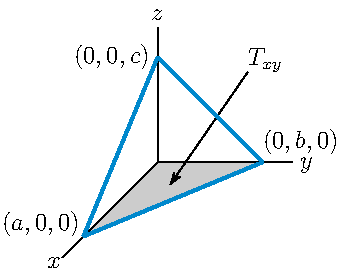
\includegraphics{triangleProjection.pdf}
\end{center}


\emph{Method 2.}\ \ \ 
 $S$ is the part of the surface $x=g(y,z)$ with 
$g(y,z) = a\left(1-\frac{y}{b}-\frac{z}{c}\right)$
and with $(y,z)$ running over the triangle $T_{yz}$ in the $yz$-plane 
with vertices $(0,0,0)$ $(0,b,0)$ and $(0,0,c)$.
Hence by the second part of (\eref{CLP317}{eq:SUdSgraph}) in the CLP-4 text,
\begin{align*}
\text{Area}(S)&=\dblInt_{T_{yz}} \sqrt{1+g_y(y,z)^2+g_z(y,z)^2}\ \dee{y}\,\dee{z} \\
&=\dblInt_{T_{yz}}\ \sqrt{1+\frac{a^2}{b^2}+\frac{a^2}{c^2}}\  
\dee{y}\,\dee{z}\\
&=\sqrt{1+\frac{a^2}{b^2}+\frac{a^2}{c^2}}\ A(T_{yz})
\end{align*}
where $A(T_{yz})$ is the area of $T_{yz}$. Since $T_{yz}$ has base $b$ and 
height $c$, it has area $\frac{1}{2}bc$. So
\begin{equation*}
\text{Area}(S)=\frac{1}{2}\sqrt{1+\frac{a^2}{b^2}+\frac{a^2}{c^2}}\ bc 
 =\frac{1}{2}\sqrt{a^2b^2+a^2c^2+b^2c^2}
\end{equation*}

\emph{Method 3.}\ \ \ 
 $S$ is the part of the surface $y=h(x,z)$ with 
$h(x,z) = b\left(1-\frac{x}{a}-\frac{z}{c}\right)$
and with $(x,z)$ running over the triangle $T_{xz}$ in the $xz$-plane 
with vertices $(0,0,0)$ $(a,0,0)$ and $(0,0,c)$.
Hence by the third part of (\eref{CLP317}{eq:SUdSgraph}) in the CLP-4 text,
\begin{align*}
\text{Area}(S)&=\dblInt_{T_{xz}} \sqrt{1+h_x(x,z)^2+h_z(x,z)^2}\ \dee{x}\,\dee{z} \\
&=\dblInt_{T_{xz}}\ \sqrt{1+\frac{b^2}{a^2}+\frac{b^2}{c^2}}\  
\dee{x}\,\dee{z}\\
&=\sqrt{1+\frac{b^2}{a^2}+\frac{b^2}{c^2}}\ A(T_{xz})
\end{align*}
where $A(T_{xz})$ is the area of $T_{xz}$. Since $T_{xz}$ has base $a$ and 
height $c$, it has area $\frac{1}{2}ac$. So
\begin{equation*}
\text{Area}(S)=\frac{1}{2}\sqrt{1+\frac{b^2}{a^2}+\frac{b^2}{c^2}}\ bc 
 =\frac{1}{2}\sqrt{a^2b^2+a^2c^2+b^2c^2}
\end{equation*}

(b) We have already seen in the solution to part (a) that
\begin{equation*}
\text{Area}(T_{xy})=\frac{ab}{2}\qquad
\text{Area}(T_{xz})=\frac{ac}{2}\qquad
\text{Area}(T_{yz})=\frac{bc}{2}\qquad
\end{equation*}
Hence
\begin{align*}
\text{Area}(S) 
&=\sqrt{\frac{a^2b^2}{4}+\frac{a^2c^2}{4}+\frac{b^2c^2}{4}} \\
&=\sqrt{\text{Area}(T_{xy})^2
                     +\text{Area}(T_{xz})^2
                     +\text{Area}(T_{yz})^2
                     }
\end{align*}

\end{solution}

%%%%%%%%%%%%%%%%%%%%%%%%%%%
\begin{question}
Let $a,h>0$. Denote by $S$ the part of the cylinder $x^2+z^2=a^2$ with 
$x\ge 0$, $0\le y\le h$ and $z\ge 0$.

\begin{center}
     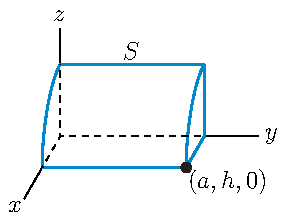
\includegraphics{cylinderQ.pdf}
\end{center}

\begin{enumerate}[(a)]
\item 
Find the surface area of $S$ without using any calculus.
\item
Parametrize $S$ by 
\begin{equation*}
\vr(\theta,y) = a\,\cos\theta\ \hi +y\,\hj +a\sin\theta\ \hk\quad
0\le\theta\le\frac{\pi}{2},\ 
0\le y\le h
\end{equation*}
Find the surface area of $S$ by using (\eref{CLP317}{eq:SUdSparam})
in the CLP-4 text.
\end{enumerate}

\end{question}

\begin{hint} 
Flatten $S$ out.
\end{hint}

\begin{answer} 
$\frac{\pi ah}{2}$
\end{answer}

\begin{solution}
(a) 
Think of the cylinder as being a piece of paper that has been partially rolled 
up. If you flatten the piece of paper out, you get a rectangle
with the length of one side being $h$ and the length of the other side
being one quarter of the circumference of a circle of radius $a$,
i.e. $\frac{1}{4}(2\pi a)=\frac{\pi a}{2}$. So the area of $S$ is
$\frac{\pi a h}{2}$.

(b) $S$ is parametrized by
\begin{equation*}
x(\theta,y)=a\cos\theta\qquad
y(\theta,y)=y\qquad
z(\theta,z)=a\sin\theta
\end{equation*}
with $(\theta,y)$ running over 
$0\le \theta\le \frac{\pi}{2},\ 0\le y\le h$. Then,
by (\eref{CLP317}{eq:SUdSparam}) in the CLP-4 text,
\begin{align*}
\Big(\pdiff{x}{\theta},\pdiff{y}{\theta},\pdiff{z}{\theta}\Big)
&=(-a\sin\theta,0,a\cos\theta)\\
\Big(\pdiff{x}{y},\pdiff{y}{y},\pdiff{z}{y}\Big)
&=(0,1,0)\\
\dee{S}
&=
 \Big|\Big(\pdiff{x}{\theta},\pdiff{y}{\theta},\pdiff{z}{\theta}\Big)
\times\Big(\pdiff{x}{y},\pdiff{y}{y},\pdiff{z}{y}\Big)\Big|
     \dee{\theta} \dee{y}\\
&=\big|(-a\cos\theta,0,-a\sin\theta)\big|\,\dee{\theta}\,\dee{y}\\
&=a\,\dee{\theta}\,\dee{y}
\end{align*}
So
\begin{align*}
\text{Area}(S)&=\dblInt_S\dee{S}
=\int_0^{\pi/2}\dee{\theta}\int_0^h\dee{y}\ a 
=a\left(\frac{\pi}{2}\right)h
\end{align*}

\end{solution}


%%%%%%%%%%%%%%%%%%
\subsection*{\Procedural}
%%%%%%%%%%%%%%%%%%

%%%%%%%%%%%%%%%%%%%%%%%%%%%%%%%%%%%
\begin{question}
Let $S$ be the part of the surface $z = xy$ lying inside the cylinder 
$x^2 + y^2 = 3$.  Find the moment of inertia of $S$ about the 
$z$-axis, that is,  
\begin{equation*}
      I =  \dblInt_S (x^2 + y^2)\ \dee{S} 
\end{equation*}
\end{question}

%\begin{hint} 
%\end{hint}

\begin{answer} 
$\frac{116}{15}\pi$
\end{answer}

\begin{solution}
The surface is $z=f(x,y)$ with $f(x,y)=xy$. So, by 
(\eref{CLP317}{eq:SUdSgraph}) in the CLP-4 text, 
\begin{equation*}
\dee{S}=\sqrt{1+f_x^2+f_y^2}\ \dee{x}\,\dee{y}
         =\sqrt{1+x^2+y^2}\ \dee{x}\,\dee{y}
\end{equation*}
and
\begin{align*}
I &=  \dblInt_S (x^2 + y^2)\ \dee{S}
  = \dblInt_{x^2+y^2\le 3} (x^2 + y^2)\ \sqrt{1+x^2+y^2}\ \dee{x}\,\dee{y} \\
  &= \int_0^{2\pi}\dee{\theta}\int_0^{\sqrt{3}} \dee{r}\ r\ r^2\sqrt{1+r^2}
\end{align*}
We switched to polar coordinates in the last step.   
Making the change of variables $u=1+r^2$, $\dee{u}=2r\,\dee{r}$
\begin{align*}
I = \pi \int_1^{4} \dee{u}\ (u-1)\sqrt{u}
=\pi\left[\frac{2}{5}u^{5/2}-\frac{2}{3}u^{3/2}\right]_1^4
=\pi\left[\frac{64}{5}-\frac{16}{3}-\frac{2}{5}+\frac{2}{3}\right]
=\frac{116}{15}\pi
\end{align*}
\end{solution}


%%%%%%%%%%%%%%%%%%%%%%%%%%%%%%%%
\begin{question}[M253 2013D] %4
Find the surface area of the part of the paraboloid 
$z = a^2 - x^2 - y^2$ which lies above the $xy$--plane.
\end{question}

%\begin{hint}
%\end{hint}

\begin{answer}
$\frac{\pi}{6}\big[{(1+4a^2)}^{3/2}-1\big]$
\end{answer}

\begin{solution}
First observe that any point $(x,y,z)$ on the paraboliod lies above the $xy$-plane if and only if
\begin{equation*}
0\le z = a^2-x^2-y^2
\iff x^2+y^2\le a^2
\end{equation*} 
That is, if and only if $(x,y)$ lies in the circular disk of radius $a$
centred on the origin. The equation of the paraboloid is of the form 
$z=f(x,y)$ with $f(x,y)=a^2-x^2-y^2$. So, by 
(\eref{CLP317}{eq:SUdSgraph}) in the CLP-4 text,
\begin{align*}
\text{Surface area}
&= \dblInt_{x^2+y^2\le a^2}\sqrt{1+f_x(x,y)^2+f_y(x,y)^2}\ \dee{x}\,\dee{y} \\
&= \dblInt_{x^2+y^2\le a^2}\sqrt{1+4x^2+4y^2}\ \dee{x}\,\dee{y}
\end{align*}
Switching to polar coordinates,
\begin{align*}
\text{Surface area}
&= \int_0^a\dee{r}\int_0^{2\pi}\dee{\theta}\ r\sqrt{1+4r^2}\\
&= 2\pi \int_0^a\dee{r}\ r\sqrt{1+4r^2}\\
&= 2\pi \int_1^{1+4a^2}\frac{\dee{s}}{8}\ \sqrt{s}\qquad
\text{with $s=1+4r^2$, $\dee{s}=8r\,\dee{r}$} \\
&=\frac{\pi}{4}\ \frac{2}{3}s^{3/2}\bigg|_{s=1}^{s=1+4a^2} \\
&=\frac{\pi}{6}\big[{(1+4a^2)}^{3/2}-1\big]
\end{align*}

\end{solution}


%%%%%%%%%%%%%%%%%%%%%%%%%%%%%%%%
\begin{question}[M253 2014D] %7a
Find the area of the portion of the cone $z^2 = x^2 + y^2$ 
lying between the planes $z = 2$ and $z = 3$.
\end{question}

%\begin{hint}
%\end{hint}

\begin{answer}
$5\sqrt{2}\pi$
\end{answer}

\begin{solution}
First observe that any point $(x,y,z)$ on the cone lies between the 
planes $z=2$ and $z=3$ if and only if $4\le x^2+y^2\le 9$.
%That is, if and only if $(x,y)$ has polar coordinate $r$ between $2$ and $3$. 
The equation of the cone can be rewritten in the form 
$z=f(x,y)$ with $f(x,y)=\sqrt{x^2+y^2}$. Note that
\begin{align*}
f_x(x,y)=\frac{x}{\sqrt{x^2+y^2}}\qquad
f_y(x,y)=\frac{y}{\sqrt{x^2+y^2}}
\end{align*}
So, by 
(\eref{CLP317}{eq:SUdSgraph}) in the CLP-4 text,
\begin{align*}
\text{Surface area}
&= \dblInt_{4\le x^2+y^2\le 9}\sqrt{1+f_x(x,y)^2+f_y(x,y)^2}\ \dee{x}\,\dee{y} \\
&= \dblInt_{4\le x^2+y^2\le 9}
    \sqrt{1+\frac{x^2}{x^2+y^2}+\frac{y^2}{x^2+y^2}}\ \dee{x}\,\dee{y} \\
&=\sqrt{2} \dblInt_{4\le x^2+y^2\le 9} \dee{x}\,\dee{y} 
\end{align*}
Now the domain of integration is a circular washer with outside radius $3$
and inside radius $2$ and hence of area $\pi(3^2-2^2)=5\pi$. So the surface area is $5\sqrt{2}\pi$.

\end{solution}
%%%%%%%%%%%%%%%%%%%%%%%%%%%%%%%%
\begin{question}[M253 2015D] %8
Determine the surface area of the surface given by 
$z = \frac{2}{3}\big(x^{3/2} + y^{3/2}\big)$, over the square
$0 \le  x \le  1$, $0 \le  y \le  1$.
\end{question}

%\begin{hint}
%\end{hint}

\begin{answer}
$\frac{4}{15}\big[9\sqrt{3}-8\sqrt{2}+1\big]$
\end{answer}

\begin{solution}
The equation of the surface is of the form 
$z=f(x,y)$ with $f(x,y)=\frac{2}{3}\big(x^{3/2} + y^{3/2}\big)$. Note that
\begin{align*}
f_x(x,y)=\sqrt{x}\qquad
f_y(x,y)=\sqrt{y}
\end{align*}
So, by (\eref{CLP317}{eq:SUdSgraph}) in the CLP-4 text,
\begin{align*}
\text{Surface area}
&= \int_0^1\dee{x}\int_0^1\dee{y}\ \sqrt{1+f_x(x,y)^2+f_y(x,y)^2} \\
&= \int_0^1\dee{x}\int_0^1\dee{y}\ \sqrt{1+x+y} \\
&= \int_0^1\dee{x}\ \Big[\frac{2}{3}(1+x+y)^{3/2}\Big]_{y=0}^{y=1} \\
&= \frac{2}{3}\int_0^1\dee{x}\ \big[(2+x)^{3/2}-(1+x)^{3/2}\big] \\
&= \frac{2}{3}\ \frac{2}{5}\Big[(2+x)^{5/2}-(1+x)^{5/2}\Big]_{x=0}^{x=1} \\
&= \frac{4}{15} \big[3^{5/2}-2^{5/2}-2^{5/2}+1^{5/2}\big] \\
&= \frac{4}{15}\big[9\sqrt{3}-8\sqrt{2}+1\big]
\end{align*}
\end{solution}

%%%%%%%%%%%%%%%%%%%%%%%%%%%%%%%%
\begin{question}[M253 2016D] %2
\begin{enumerate}[(a)]
\item
To find the surface area of the surface $z = f (x,y)$ above the region $D$, 
we integrate $\dblInt_D F(x,y)\ \dee{A}$. What is $F(x,y)$?
\item
Consider a ``Death Star'',  a ball of radius $2$ centred at the origin 
with another ball of radius $2$ centred at $(0, 0, 2\sqrt{3})$ cut out of it. 
The diagram below shows the slice where $y = 0$.

\begin{center}
     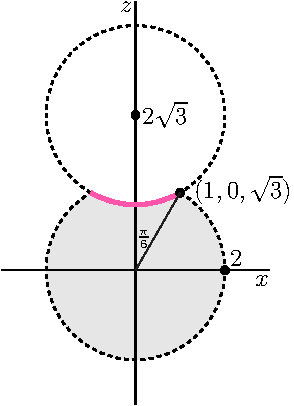
\includegraphics{OE253_16D_2.pdf}
\end{center}

\begin{enumerate}[(i)]
\item
The Rebels want to paint part of the surface of Death Star hot pink; specifically, the concave part (indicated with a thick line in the diagram). 
To help them determine how much paint is needed, carefully fill in the 
missing parts of this integral:
\begin{equation*}
\text{surface area} = 
\int_{\underline{\ \ \ \ }}^{\underline{\ \ \ \ }}
                 \int_{\underline{\ \ \ \ }}^{\underline{\ \ \ \ }}
                        \underline{\ \ \ \ \ \ \ \ \ \ }\ \dee{r}\,\dee{\theta}
\end{equation*}

\item
What is the total surface area of the Death Star?
\end{enumerate}
\end{enumerate}
\end{question}

\begin{hint}
The total surface area of (b) (ii) can be determined without evaluating
any integrals.
\end{hint}

\begin{answer}
(a)  $F(x,y) = \sqrt{1+f_x(x,y)^2+f_y(x,y)^2}$
\qquad
(b) (i) $\int_0^{2\pi}\dee{\theta}\int_0^1\dee{r}\ \frac{2r}{\sqrt{4-r^2}}$ 
\qquad (ii) $\frac{32\pi}{3}$
\end{answer}

\begin{solution}
(a)
By (\eref{CLP317}{eq:SUdSgraph}) in the CLP-4 text,
$F(x,y) = \sqrt{1+f_x(x,y)^2+f_y(x,y)^2}$.

(b)  (i) The ``dimple'' to be painted is part of the upper sphere
$x^2+y^2+\big(z-2\sqrt{3}\big)^2=4$. It is on the bottom half of the sphere
and so has equation $z=f(x,y)=2\sqrt{3}-\sqrt{4-x^2-y^2}$. Note that
\begin{align*}
f_x(x,y) = \frac{x}{\sqrt{4-x^2-y^2}}\qquad
f_y(x,y) = \frac{y}{\sqrt{4-x^2-y^2}}
\end{align*}
The point on the dimple with the largest value of $x$ is
$(1,0,\sqrt{3})$. (It is marked by a dot in the figure above.) The dimple
is invariant under rotations around the $z$--axis and so has $(x,y)$
running over $x^2+y^2\le 1$. So, by 
(\eref{CLP317}{eq:SUdSgraph}) in the CLP-4 text,
\begin{align*}
\text{Surface area}
&= \dblInt_{x^2+y^2\le 1}\sqrt{1+f_x(x,y)^2+f_y(x,y)^2}\ \dee{x}\,\dee{y} \\
&= \dblInt_{x^2+y^2\le 1}\sqrt{1+\frac{x^2}{4-x^2-y^2}
                                +\frac{y^2}{4-x^2-y^2}}\ \dee{x}\,\dee{y} \\
&= \dblInt_{x^2+y^2\le 1}\frac{2}{\sqrt{4-x^2-y^2}}\ \dee{x}\,\dee{y} 
\end{align*}
Switching to polar coordinates,
\begin{align*}
\text{Surface area}
&= \int_0^{2\pi}\dee{\theta}\int_0^1\dee{r}\ \frac{2r}{\sqrt{4-r^2}}
\end{align*}

(b) (ii) Observe that if we flip the dimple up by reflecting it
in the plane $z=\sqrt{3}$, as in the figure below, the ``Death Star'' 
becomes a perfect ball of radius $2$.  
\begin{center}
     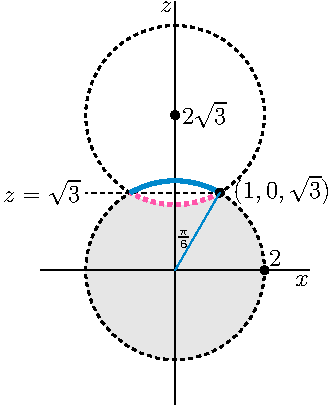
\includegraphics{OE253_16D_2a.pdf}
\end{center}
The area of the pink dimple in the figure above is identical to the area
of the blue cap in that figure. So the total surface area of the 
Death Star is exactly the surface area of a sphere of radius $2$ and so
is $\frac{4}{3}\pi 2^3=\frac{32\pi}{3}$.

\end{solution}

%%%%%%%%%%%%%%%%%%%%%%%%%%%%%%%%%%%%%%%%%
\begin{question} [M200 2003A] % 7b
Find the area of the cone $z^2=x^2+y^2$ between $z=1$ and $z=16$.
\end{question}

%\begin{hint}
%
%\end{hint}

\begin{answer}
$255\sqrt{2}\pi\approx 1132.9$
\end{answer}

\begin{solution}
On the upper half of the cone 
\begin{equation*}
z=f(x,y)=\sqrt{x^2+y^2}\qquad 
f_x(x,y)=\frac{x}{\sqrt{x^2+y^2}}\qquad
f_y(x,y)=\frac{y}{\sqrt{x^2+y^2}}
\end{equation*}
so that
\begin{equation*}
\dee{S}=\sqrt{1+f_x(x,y)^2+f_y(x,y)^2}\,\dee{x}\,\dee{y}
=\sqrt{1+\frac{x^2}{x^2+y^2}+\frac{y^2}{x^2+y^2}}\,\dee{x}\,\dee{y}
=\sqrt{2}\,\dee{x}\,\dee{y}
\end{equation*}
and
\begin{align*}
\text{Area}&= \dblInt_{1\le x^2+y^2\le 16^2}\sqrt{2}\,\dee{x}\,\dee{y} \\
&=\sqrt{2}\,\Big[\text{area of }\Set{(x,y)}{x^2+y^2\le 16^2}-
           \text{area of }\Set{(x,y)}{x^2+y^2\le 1}\Big] \\
&=\sqrt{2}\,\big[\pi 16^2-\pi 1^2\big]
=255\sqrt{2}\pi\approx 1132.9
\end{align*}
\end{solution}

%%%%%%%%%%%%%%%%%%%%%%%%%%%%%%%%%%%%%%%%%
\begin{question} [M200 2001D] %7
Find the surface area of that part of the hemisphere 
$z=\sqrt{a^2-x^2-y^2}$ which lies within the cylinder $\big(x-\frac{a}{2}\big)^2+y^2=\big(\frac{a}{2}\big)^2$.
\end{question}

%\begin{hint}
%
%\end{hint}

\begin{answer}
$a^2[\pi-2]$
\end{answer}

\begin{solution}
We are to find the surface area of part of a hemisphere. On the hemisphere 
\begin{align*}
z=f(x,y)=\sqrt{a^2-x^2-y^2}\qquad 
f_x(x,y)=-\frac{x}{\sqrt{a^2-x^2-y^2}}\qquad
f_y(x,y)=-\frac{y}{\sqrt{a^2-x^2-y^2}}
\end{align*}
so that
\begin{align*}
\dee{S}&=\sqrt{1+f_x(x,y)^2+f_y(x,y)^2}\,\dee{x}\,\dee{y}
=\sqrt{1+\frac{x^2}{a^2-x^2-y^2}+\frac{y^2}{a^2-x^2-y^2}}\,\dee{x}\,\dee{y} \\
&=\sqrt{\frac{a^2}{a^2-x^2-y^2}}\,\dee{x}\,\dee{y}
\end{align*}
In polar coordinates, this is $\dee{S}=\frac{a}{\sqrt{a^2-r^2}}\,r\,\dee{r}\,\dee{\theta}$.
We are to find the surface area of the part of the hemisphere that is 
inside the cylinder, $x^2-ax+y^2=0$, which is polar coordinates is
becomes $r^2-ar\cos\theta=0$ or $r=a\cos\theta$. The top half of the domain of
integration is sketched below.  
\begin{center}
     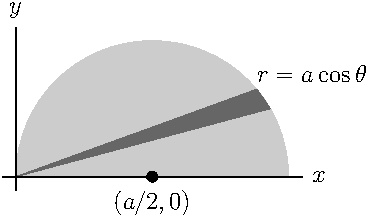
\includegraphics{OE01DQ7.pdf}
\end{center}
So the
\begin{align*}
{\rm Surface\ Area}
&= 2\int_0^{\pi/2}\dee{\theta}\int_0^{a\cos\theta}\dee{r}\ r
                                      \frac{a}{\sqrt{a^2-r^2}}
= 2a\int_0^{\pi/2}\dee{\theta}\ \Big[-\sqrt{a^2-r^2}\,\Big]_0^{a\cos\theta}
\\
&= 2a\int_0^{\pi/2}\dee{\theta}\ \big[a-a\sin\theta\big] \\
&= 2a^2\Big[\theta+\cos\theta\Big]_0^{\pi/2}
=a^2[\pi-2]
\end{align*}
\end{solution}




%%%%%%%%%%%%%%%%%%%%%%%%%%%
\begin{question}
The cylinder $\ x^2+y^2=2x\ $ cuts out a portion 
$S$ of the upper half of the cone $\ x^2+y^2=z^2$. Compute
\begin{equation*}
\dblInt_S(x^4-y^4+y^2z^2-z^2x^2+1)\,\dee{S}
\end{equation*}
\end{question}

\begin{hint} 
On $S$, $(x,y)$ runs over the interior of $x^2+y^2=2x$,
or equivalently, the interior of $(x-1)^2+y^2=1$.
\end{hint}

\begin{answer} 
$\sqrt{2}\ \pi$
\end{answer}

\begin{solution} 
The upper half cone obeys $f(x,y,z)=x^2+y^2-z^2=0$. So,
by (\eref{CLP317}{eq:SUdSimplicit}) in the CLP-4 text,
\begin{equation*}
\dee{S}=\left|\frac{\vnabla f}{\vnabla f\cdot\hk}\right|\dee{x}\,\dee{y}
=\left|\frac{2x\hi+2y\hj-2z\hk}{-2z}\right|\dee{x}\,\dee{y}
=\frac{\sqrt{x^2+y^2+z^2}}{z}\dee{x}\,\dee{y}
\end{equation*}
But on the cone $x^2+y^2=z^2$, and $z>0$, so that
\begin{equation*}
\dee{S}=\frac{\sqrt{x^2+y^2+z^2}}{z}\dee{x}\,\dee{y}
=\frac{\sqrt{2z^2}}{z}\dee{x}\,\dee{y}
=\sqrt{2}\,\dee{x}\,\dee{y}
%=\sqrt{2}r\,\dee{r}\,\dee{\theta}
\end{equation*}
and
\begin{align*}
x^4-y^4+y^2z^2-z^2x^2+1
&=x^4-y^4+y^2\big(x^2+y^2\big)-\big(x^2+y^2)x^2+1
=1
\end{align*}
We have to integrate $(x,y)$ over the interior of $x^2+y^2=2x$,
or equivalently, the interior of $(x-1)^2+y^2=1$,
which is the disk
\begin{equation*}
D=\Set{(x,y)}{(x-1)^2+y^2\le 1}
\end{equation*}
So
\begin{align*}
\dblInt_S\overbrace{(x^4-y^4+y^2z^2-z^2x^2+1)}^{=1}\,\dee{S}
&=\sqrt{2}\dblInt_D \dee{x}\,\dee{y}
=\sqrt{2}\ \text{Area}(D)
=\sqrt{2}\ \pi
\end{align*}
\end{solution}

%%%%%%%%%%%%%%%%%%%%%%%%%%%
\begin{question}
Find the surface area of the torus obtained by rotating the
circle $(x-R)^2+z^2=r^2$ (the circle is contained in the $xz$-plane)
 about the $z$-axis.
\end{question}

\begin{hint} 
See Example \eref{CLP317}{SURdonut} of the CLP-4 text for a parametrization
of the torus.
\end{hint}

\begin{answer} 
$(2\pi)^2 Rr$
\end{answer}

\begin{solution} 
As we saw in Example \eref{CLP317}{SURdonut} of the CLP-4 text,
the torus may be parametrized by
\begin{equation*}
\vr(\theta,\psi)
  = (R+r\cos\theta)\cos\psi\,\hi
    +(R+r\cos\theta)\sin\psi\,\hj
    + r\sin\theta\,\hk\qquad
0\le\theta,\psi\le 2\pi
\end{equation*}
Then
\begin{equation*}
\pdiff{\vr}{\psi}=(R+r\cos\theta)\big[-\sin\psi\hi+\cos\psi\hj\big]\qquad
\pdiff{\vr}{\theta}=r\big[-\sin\theta\cos\psi\,\hi-\sin\theta\sin\psi\,\hj
               +\cos\theta\,\hk\big]
\end{equation*}
and
\begin{align*}
\pdiff{\vr}{\psi}\times\pdiff{\vr}{\theta}
&=r(R+r\cos\theta)\ \big[-\sin\psi\hi+\cos\psi\hj\big]\times
           \big[-\sin\theta\cos\psi\,\hi-\sin\theta\sin\psi\,\hj
               +\cos\theta\,\hk\big] \\
&=r(R+r\cos\theta)\det\left[\begin{matrix}
                 \hi   &   \hj               &   \hk   \\
            -\sin\psi  & \cos\psi            & 0       \\
   -\sin\theta\cos\psi & -\sin\theta\sin\psi & \cos\theta 
    \end{matrix}\right] \\
&=r(R+r\cos\theta) \big[\cos\psi\cos\theta\,\hi +\sin\psi\cos\theta\,\hj
                          +\sin\theta\,\hk\big]
\end{align*}
As $\big[\cos\psi\cos\theta\,\hi +\sin\psi\cos\theta\,\hj
                          +\sin\theta\,\hk\big]$ is a unit vector,
(we could have shortened this computation by observing that $-\sin\psi\,\hi+\cos\psi\,\hj$ and
 $-\sin\theta\cos\psi\,\hi-\sin\theta\sin\psi\,\hj+\cos\theta\,\hk$ 
are mutually perpendicular unit vectors, so that their cross product is 
automatically a unit vector) and
\begin{equation*}
\left|\pdiff{\vr}{\psi}\times\pdiff{\vr}{\theta}\right|
=r(R+r\cos\theta)
\implies \dee{S}=r(R+r\cos\theta)\,d\psi\,\dee{\theta}
\end{equation*}
The total surface area of the torus is
\begin{equation*}
r\int_0^{2\pi}\dee{\theta}\int_0^{2\pi}d\psi\,(R+r\cos\theta)
=2\pi r \int_0^{2\pi}\dee{\theta}\,(R+r\cos\theta)
=(2\pi)^2 Rr
\end{equation*}
\end{solution}

%%%%%%%%%%%%%%%%%%%%%%%%%%%
\begin{question}
A spherical shell of radius $a$ is centred at the origin.
Find the centroid (i.e. the centre of mass with constant density)
of the part of the sphere that lies in the first octant.
\end{question}

\begin{hint}
Call the part of the sphere in the first octant $S$.
By definition, the centroid is  $(\bar x,\bar y,\bar z)$ with
\begin{equation*}
\bar x = \frac{\dblInt_S x\ \dee{S}}{\dblInt_S \ \dee{S}}\qquad
\bar y = \frac{\dblInt_S y\ \dee{S}}{\dblInt_S \ \dee{S}}\qquad
\bar z = \frac{\dblInt_S z\ \dee{S}}{\dblInt_S \ \dee{S}}
\end{equation*}
The integrals will be easy if you use spherical coordinates.
You can reduce the number of integrals evaluated by using symmetry.
\end{hint}

\begin{answer} 
$\left(\frac{a}{2}\,,\,\frac{a}{2}\,,\,\frac{a}{2}\right)$
\end{answer}

\begin{solution} 
By symmetry, the centroid $(\bar x,\bar y,\bar z)$
obeys $\bar x=\bar y=\bar z$. Parametrize the sphere
using spherical coordinates.
\begin{equation*}
\vr(\theta,\varphi) = a\sin\varphi\cos\theta\,\hi 
                     +a\sin\varphi\sin\theta\,\hj
                     +a\cos\varphi\,\hk
\end{equation*}
Then
\begin{align*}
\pdiff{\vr}{\theta}
       =-a\sin\varphi\sin\theta\,\hi+a\sin\varphi\cos\theta\,\hj\qquad
\pdiff{\vr}{\varphi}
       =a\cos\varphi\cos\theta\,\hi+a\cos\varphi\sin\theta\,\hj
               -a\sin\varphi\,\hk
\end{align*}
so that
\begin{align*}
\pdiff{\vr}{\theta}\times\pdiff{\vr}{\varphi}
&=\det\left[\begin{matrix}
                    \hi   &       \hj               &   \hk   \\
  -a\sin\varphi\sin\theta & a\sin\varphi\cos\theta  & 0       \\
   a\cos\varphi\cos\theta & a\cos\varphi\sin\theta  & -a\sin\varphi
    \end{matrix}\right] 
\\
&=-a^2\sin^2\varphi\cos\theta\,\hi-a^2\sin^2\varphi\sin\theta\,\hj
           -a^2\sin\varphi\cos\varphi\,\hk\\
\implies \dee{S}&=\left|\pdiff{\vr}{\theta}\times\pdiff{\vr}{\varphi}\right|
              \,\dee{\theta}\,\dee{\varphi}
           =a^2\sin\varphi\,\dee{\theta}\,\dee{\varphi}
\end{align*}
As the surface area of the part of the sphere in the first octant is
$\frac{1}{8}4\pi a^2=\frac{\pi a^2}{2}$
\begin{align*}
\bar x=\bar y=\bar z
&=\frac{\dblInt_S z\,\dee{S}}{\dblInt_S\,\dee{S}}
=\frac{1}{\pi a^2/2}\int_0^{\pi/2}\dee{\theta}\int_0^{\pi/2}\dee{\varphi} \ 
(a^2\sin\varphi)(\overbrace{a\cos\varphi}^{z}) \\
&=\frac{2a}{\pi}\frac{\pi}{2}\int_0^{\pi/2}\dee{\varphi} \ \sin\varphi\cos\varphi 
=a\bigg[\frac{1}{2}\sin^2\varphi\bigg]_0^{\pi/2}
=\frac{a}{2}
\end{align*}
\end{solution}

%%%%%%%%%%%%%%%%%%%%%%%%%%%
\begin{question}
Find the area of
 that part of the cylinder $x^2+y^2=2ay$ lying outside $z^2=x^2+y^2$. 
\end{question}

\begin{hint}
Before parametrizing the cylinder, express
$x^2+y^2=2ay$ in cylindrical coordinates. 
\end{hint}

\begin{answer} 
$16a^2$
\end{answer}

\begin{solution} 
In cylindrical coordinates
\begin{equation*}
x=r\cos\theta\qquad
y=r\sin\theta\qquad
z=z
\end{equation*}
In these coordinates the equation, $x^2+y^2=2ay$, of the cylinder
becomes
\begin{equation*}
r^2=2ar\sin\theta\qquad\text{or}\qquad r=2a\sin\theta
\end{equation*}
That is, $r=f(\theta)$ with $f(\theta) =2a\sin\theta$.
Parametrize the cylinder by 
$\vr(\theta,z) = x(\theta,z)\,\hi + y(\theta,z)\,\hj + z(\theta,z)\,\hk$
with
\begin{align*}
x(\theta,z)&=f(\theta)\cos\theta=2a\sin\theta\cos\theta=a\sin2\theta\\
y(\theta,z)&=f(\theta)\sin\theta=2a\sin\theta\sin\theta=a(1-\cos2\theta)\\
z(\theta,z)&=z
\end{align*}
Under this parametrization,
\begin{align*}
\pdiff{\vr}{\theta}=2a\cos2\theta\,\hi+2a\sin2\theta\,\hj\qquad
\pdiff{\vr}{z}=\hk
&\implies \pdiff{\vr}{\theta}\times\pdiff{\vr}{z}
=-2a\cos2\theta\,\hj+2a\sin2\theta\,\hi \\
&\implies \dee{S}=\left|\pdiff{\vr}{\theta}\times\pdiff{\vr}{z}\right|\,
                         \dee{\theta}\,\dee{z}
                 =2a\,\dee{\theta}\,\dee{z}
\end{align*}
We still have to determine the limits of integration.
The figure on the left below provides a top view of the cylinder.
\begin{center}
          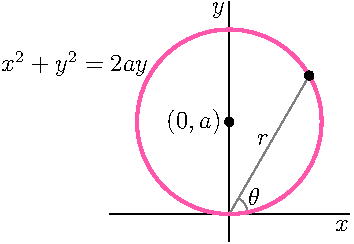
\includegraphics{coneCylA.pdf}\qquad\qquad
          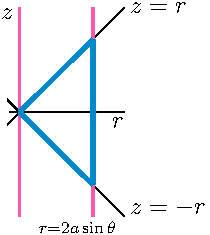
\includegraphics{coneCyl.pdf}
\end{center}
From it we see that $0\le\theta\le\pi$.
The cone $z^2=x^2+y^2=r^2$ (i.e. $z=\pm r$)
and the cylinder $r=2a\sin\theta$ intersect at
$z^2=r^2=4a^2\sin^2\theta$. 
So, for each fixed $\theta$, $z$ runs from $-2a\sin\theta$ to $z=+2a\sin\theta$.
(See the figure on the right above. It shows a constant $\theta$
cross-section.) Finally,
\begin{align*}
{\rm Area} &= \int_{|z|\le 2a\sin\theta}2a\,\dee{\theta}\,\dee{z}
=2a\int_0^\pi \!\!\dee{\theta}\int_{-2a\sin\theta}^{2a\sin\theta} \!\!\!\dee{z}
=8a^2\int_0^\pi \!\!\dee{\theta}\ \sin\theta
=8a^2\Big[-\cos\theta\Big]_0^\pi \\
&=16a^2
\end{align*}
\end{solution}

%%%%%%%%%%%%%%%%%%%%%%%%%%%
\begin{question}[M317 2000D] %3
Let $a$ and $b$ be positive constants, and let $\cS$ be
the part of the conical surface
$$
a^2 z^2 = b^2(x^2+y^2)
$$
where $0\le z\le b$.
Consider the surface integral
$$
I = \dblInt_\cS (x^2+y^2)\,\dee{S}.
$$
\begin{enumerate}[(a)]
\item
Express $I$ as a double integral over a disk
in the $xy$-plane.

\item
Use the parametrization $x=t\cos\theta$, $y=t\sin\theta$, etc.,
to express $I$ as a double integral over a suitable region in the
$t\theta$-plane.

\item
Evaluate $I$ using the method of your choice.
\end{enumerate}

\end{question}

%\begin{hint} 
%\end{hint}

\begin{answer} 
$\frac{\pi}{ 2}a^3\sqrt{a^2+b^2}$
\end{answer}

\begin{solution} 
(a)
This right circular cone symmetric about the $z$-axis projects down
onto a disk $\cD$ in the plane $z=0$.  Setting $z=b$ gives
$$
\cD=\Set{(x,y,z)}{x^2 + y^2 \le a^2,\  z=0}
$$
Since $G(x,y,z) = b^2(x^2+y^2)-a^2z^2$ is constant on $\cS$, the
area elements $\dee{S}$ on $\cS$ are related to area elements 
$\dee{x}\dee{y}$ on $\cD$ as follows:
$$
\dee{S} = \frac{|\nabla G(x,y,z)|}{ |\nabla G(x,y,z)\cdot\hk|}\,\dee{x}\dee{y}
= \frac{2|(b^2 x,b^2 y,-a^2 z)|}{2|a^2z|}\,\dee{x}\dee{y}
= \frac{\sqrt{b^4(x^2+y^2)+a^4 z^2}}{ a^2 z}\,\dee{x}\dee{y}
$$
by (\eref{CLP317}{eq:SUdSimplicit}) in the CLP-4 text.
The defining equation for $\cS$ gives $z=\frac{b}{ a}\sqrt{x^2+y^2}$,
so
$$
\dee{S}
= \frac{\sqrt{b^4(x^2+y^2)+a^2 b^2(x^2+y^2)}}{ a\sqrt{b^2(x^2+y^2)}}\,\dee{x}\dee{y}
= \frac{1}{ a}\sqrt{a^2+b^2}\,\dee{x}\dee{y}.
$$
Hence $I = \frac{\sqrt{a^2+b^2}}{ a}\dblInt_\cD(x^2+y^2)\,\dee{x}\dee{y}$.

(b)
Or, parametrize the surface $\cS$ using $\theta$ and $t$ as
follows:
\begin{equation}
x = t\cos\theta,\
y=t\sin\theta,\ 
z = \frac{b}{ a}\sqrt{x^2+y^2} = \frac{b}{ a}t,
\qquad
0\le\theta\le 2\pi,\ 0\le t\le a.
\tag{$*$}
\end{equation}
Then we have, by (\eref{CLP317}{eq:SUdSparam}) in the CLP-4 text,
\begin{align*}
&\frac{\partial\vr}{\partial t}\times\frac{\partial\vr}{\partial\theta}
= \det\left[\begin{matrix} \hi & \hj & \hk \\
\cos\theta & \sin\theta & b/a \\
-t\sin\theta & t\cos\theta & 0 \end{matrix}\right]
= \big(-\frac{b}{ a}t\cos\theta, -\frac{b}{ a}t\sin\theta, t\big),
\\
{\rm so}\quad
&\dee{S} = \Big|\frac{\partial\vr}{\partial t}\times
            \frac{\partial\vr}{\partial\theta}\Big|\,\dee{t}\,\dee{\theta}
= t\sqrt{1+b^2/a^2}\,\dee{t}\,\dee{\theta}.
\end{align*}
It follows that for the rectangular region $\cR$ of the
$t\theta$-plane described in~$(*)$,
$$
I = \dblInt_\cR \big(t^2\big)t\sqrt{1+b^2/a^2}\,\dee{t}\,\dee{\theta}.
$$

(c)
Using polar coordinates in~(a) would give
$$
I
= \frac{\sqrt{a^2+b^2}}{ a}
  \int_{\theta=0}^{2\pi} \int_{r=0}^a r^2\,r\,\dee{r}\,\dee{\theta}
=\frac{\pi}{ 2}a^3\sqrt{a^2+b^2}.
$$
Direct integration in~(b) gives the same thing, because
$$
I
= \dblInt_\cD \big(t^2\big)t\sqrt{1+b^2/a^2}\,\dee{t}\,\dee{\theta}
= \frac{\sqrt{a^2+b^2}}{ a}\int_{\theta=0}^{2\pi} \int_{t=0}^a
t^3\,\dee{t}\,\dee{\theta}.
$$
\end{solution}


%%%%%%%%%%%%%%%%%%%%%%%%%%%
\begin{question} 
Evaluate, for each of the following,
 the flux $\ \dblInt_S\vF\cdot\hn \,\dee{S}\ $ where $\hn$ is
the outward normal to the surface $S$.
\begin{enumerate}[(a)]
\item
$\ \vF={(x^2+y^2+z^2)}^n(x\,\hi+y\,\hj+z\,\hk)\ $ 
and the surface $S$ is the sphere $x^2+y^2+z^2=a^2$.
\item
$\ \vF=x\,\hi+y\,\hj+z\,\hk\ $ 
and $S$ is the surface of the rectangular box $0\le x\le a$, $0\le y\le
b$, $0\le z\le c$.
\item
$\ \vF=y\,\hi+z\,\hk\ $ 
and $S$ is the surface of the solid cone $0\le z\le 1-\sqrt{x^2+y^2}$.
\end{enumerate}
\end{question}

\begin{hint} 
(a) The integral can be easily evaluated by using that the sphere 
has surface area $4\pi a^2$.

(c) Use cylindrcial coordinates for the top part of the cone.
\end{hint}

\begin{answer} 
(a) $4\pi a^{2n+3}$\qquad
(b) $3abc$\qquad
(c) $\frac{\pi}{3}$
\end{answer}

\begin{solution} 
(a) The surface is $g(x,y,z)=x^2+y^2+z^2-a^2=0$. So,
on the surface of the sphere,
\begin{align*}
\hn =\frac{\vnabla g}{|\vnabla g|}=\frac{x\hi+y\hj+z\hk}{\sqrt{x^2+y^2+z^2}}
&\ \Rightarrow\   \vF\cdot\hn = \big(x^2+y^2+z^2\big)^{n++1-1/2}
={\big(a^2\big)}^{n+1/2}=a^{2n+1}\\
&\ \Rightarrow\  \dblInt_S\vF\cdot\hn \,\dee{S}\ =a^{2n+1}\dblInt_S\,\dee{S}
=a^{2n+1}\text{Area}(S)
=4\pi a^{2n+3}
\end{align*}
since the surface area of a sphere of radius $a$ is $4\pi a^2$.

(b) The box has six faces.
\begin{align*}
S_1&=\Set{(x,y,z)}{0\le x\le a,\ 0\le y\le b,\ z=c}\quad
   \text{with outward normal $\hn=\hk$} \\
S_2&=\Set{(x,y,z)}{0\le x\le a,\ 0\le y\le b,\ z=0}\quad
   \text{with outward normal $\hn=-\hk$} \\
S_3&=\Set{(x,y,z)}{0\le x\le a,\ 0\le z\le c,\ y=b}\quad
   \text{with outward normal $\hn=\hj$} \\
S_4&=\Set{(x,y,z)}{0\le x\le a,\ 0\le z\le c,\ y=0}\quad
   \text{with outward normal $\hn=-\hj$} \\
S_5&=\Set{(x,y,z)}{0\le y\le b,\ 0\le z\le c,\ x=a}\quad
   \text{with outward normal $\hn=\hi$} \\
S_6&=\Set{(x,y,z)}{0\le y\le b,\ 0\le z\le c,\ x=0}\quad
   \text{with outward normal $\hn=-\hi$} 
\end{align*}
\begin{center}
       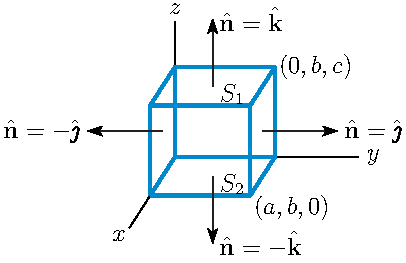
\includegraphics{cubeDTT.pdf}
\end{center}
For $S_1$, i.e. the $z=c$ face, and $S_2$, i.e. the $z=0$ face,
\begin{alignat*}{3}
\int_{\Atop{z=c}{\rm face}}\vF\cdot\hn\, \dee{S}
&=\int_{\Atop{z=c}{\rm face}}\big(x\,\hi+y\,\hj+c\,\hk\big)\cdot \hk \  \dee{x}\,\dee{y}
&&=c\int_{\Atop{z=c}{\rm face}}\dee{x}\,\dee{y}
=abc
\\
\int_{\Atop{z=0}{\rm face}}\vF\cdot\hn\, \dee{S}
&=\int_{\Atop{z=0}{\rm face}}\big(x\,\hi+y\,\hj+0\,\hk\big)\cdot(-\hk)\  \dee{x}\,\dee{y}
&&=0
\end{alignat*}
because the $z=c$ face has area $ab$.
Similarly,
$$
\int_{\Atop{x=0}{\rm face}}\vF\cdot\hn\, \dee{S}
=\int_{\Atop{y=0}{\rm face}}\vF\cdot\hn\, \dee{S}
=0\qquad
\int_{\Atop{x=a}{\rm face}}\vF\cdot\hn\, \dee{S}
=\int_{\Atop{y=b}{\rm face}}\vF\cdot\hn\, \dee{S}
=abc
$$
The total flux is $3abc$.

(c)
The base of the cone is $\Set{(x,y,z)}{x^2+y^2\le1,\ z=0}$
and has (outward) normal $\hn=-\hk$. So
The flux through the base is
\begin{equation*}
\int_{{\rm base}}\vF\cdot\hn\, \dee{S}
=\dblInt_{x^2+y^2\le 1}(y\hi)\cdot(-\hk)\,\dee{x}\,\dee{y}=0
\end{equation*}
In cylindrical coordinates
$x=r\cos\theta$,
$y=r\sin\theta$,
$z=z$
and the equation $z=1-\sqrt{x^2+y^2}$ of the top part of the cone
becomes $z=1-r$. So we may parametrize the top part of the cone by 
\begin{equation*}
\vr(r,\theta)=r\cos\theta\,\hi+r\sin\theta\,\hj
+(1-r)\,\hk
\qquad\text{with } 0\le\theta\le 2\pi,\ 0\le r\le 1
\end{equation*}
Then
\begin{align*}
\pdiff{\vr}{r}&=\cos\theta\,\hi+\sin\theta\,\hj-\hk\\
\pdiff{\vr}{\theta}&=-r\sin\theta\,\hi+r\cos\theta\,\hj\\
\pdiff{\vr}{r}\times\pdiff{\vr}{\theta}
&=\det\left[\begin{matrix}
                    \hi   & \hj   & \hk \\
               \cos\theta & \sin\theta & -1 \\
               -r\sin\theta & r\cos\theta & 0 \end{matrix}\right] \\
&= -r\cos\theta\,\hi-r\sin\theta\,\hj+r\,\hk \\
\implies \hn\,\dee{S}&=\pdiff{\vr}{r}\times\pdiff{\vr}{\theta}
                      \, \dee{r}\,\dee{\theta} \\
&=\big(-r\cos\theta\,\hi-r\sin\theta\,\hj+r\hk\big)\, \dee{r}\,\dee{\theta}
\end{align*}
by (\eref{CLP317}{SUR:paramGraph}) in the CLP-4 text.
We have the orientation correct because the $\hk$ component of $\hn$ is
positive. The flux through the top, as well as the total flux, is
\begin{align*}
\int_{{\rm top}}\vF\cdot\hn\, \dee{S}
&=\int_0^1 \dee{r}\int_0^{2\pi}\dee{\theta}\ 
                   \big(\overbrace{r\sin\theta}^{y}\,\hi
                   +\overbrace{(1-r)}^{z}\,\hk\big)
\cdot\big(-r\cos\theta\,\hi-r\sin\theta\,\hj+r\,\hk\big)\\
&=\int_0^1 \dee{r}\int_0^{2\pi}\dee{\theta}\ \big(-r^2\sin\theta\cos\theta+r(1-r)\big)
\\
&= -\bigg[\int_0^1 \dee{r}\ r^2\bigg]
         \bigg[\int_0^{2\pi}\dee{\theta}\ \frac{1}{2}\sin(2\theta)\bigg]
   +2\pi \int_0^1 \dee{r}\big[r-r^2\big] \\
&=-\frac{1}{3}\times 0+2\pi\Big[\frac{1}{2}-\frac{1}{3}\Big]
=\frac{\pi}{3}
\end{align*}
\end{solution}







%%%%%%%%%%%%%%%%%%%%%%%%%%%
\begin{question}[M317 2000A] %4
 Let $\cS$ be the part of the surface $x^2+y^2+2z=2$ that
lies above the square $-1\le x\le 1$, $-1\le y\le 1$.
\begin{enumerate}[(a)]
\item
Find $\dst\dblInt_\cS \frac{x^2+y^2}{\sqrt{1+x^2+y^2}}\ \dee{S}$.
\item
Find the flux of $\vF=x\hi+y\hj+z\hk$ upward through $\cS$.
\end{enumerate}
\end{question}

%\begin{hint} 
%\end{hint}

\begin{answer} 
(a) $\frac{8}{3}$\qquad
(b) $\frac{16}{3}$
\end{answer}

\begin{solution} 
Let $G(x,y,z) = x^2+y^2+2z$. Then, 
by (\eref{CLP317}{eq:SUdSimplicit}) of the CLP-4 text,
\begin{align*}
\hn\,\dee{S}&=\frac{\vnabla G}{\vnabla G\cdot\hk}\ \dee{x}\dee{y}
=\frac{2x\hi+2y\hj+2\hk}{2}\,\dee{x}\dee{y}
=(x\hi+y\hj+\hk)\,\dee{x}\dee{y} \\
\frac{x^2+y^2}{\sqrt{1+x^2+y^2}}\ \dee{S}
&=\frac{x^2+y^2}{\sqrt{1+x^2+y^2}}\ \sqrt{1+x^2+y^2}\,\dee{x}\dee{y}
=(x^2+y^2)\ \dee{x}\dee{y}\\
\vF\cdot\hn\,\dee{S}
&=\big[x\hi+y\hj+z\hk\big]\cdot\big[x\hi+y\hj+\hk\big]\,\dee{x}\dee{y}
=\big[x^2+y^2+z\big]\,\dee{x}\dee{y} \\
&=\Big[1+\frac{1}{2}(x^2+y^2)\Big]\,\dee{x}\dee{y}
\end{align*}
since $z=1-\half(x^2+y^2)$ on $\cS$.

(a)
\begin{align*}
\dblInt_\cS \frac{x^2+y^2}{\sqrt{1+x^2+y^2}}\ \dee{S}
&=\dblInt_\cS (x^2+y^2)\ \dee{x}\dee{y}
=4\int_0^1\dee{x}\int_0^1\dee{y}\ (x^2+y^2) \\
&=4\int_0^1\dee{x}\ \big(x^2+\frac{1}{3}\big)
=4\Big(\frac{1}{3}+\frac{1}{3}\Big)
=\frac{8}{3}
\end{align*}

(b)
$$
\dblInt_\cS \vF\cdot\hn\,\dee{S}
=\int_{-1}^1\dee{x}\int_{-1}^1\dee{y}\ \Big[1+\frac{1}{2}(x^2+y^2)\Big]
=2\times 2+\frac{1}{2}\times\frac{8}{3}
=\frac{16}{3}
$$
\end{solution}

%%%%%%%%%%%%%%%%%%%%%%%%%%%
\begin{question}[M317 1999A] %3
Let $\cS$ be the part of the surface $z=xy$ that
lies above the square $0\le x\le 1$, $0\le y\le 1$ in the $xy$-plane.
\begin{enumerate}[(a)]
\item
Find $\dst\dblInt_\cS \frac{x^2y}{\sqrt{1+x^2+y^2}}\ \dee{S}$.
\item
Find the flux of $\vF=x\hi+y\hj+\hk$ upward through $\cS$.
\end{enumerate}
\end{question}

%\begin{hint} 
%\end{hint}

\begin{answer} 
(a) $\frac{1}{6}$\qquad
(b) $\frac{1}{2}$
\end{answer}

\begin{solution} 
 Let $G(x,y,z) = z-xy$. Then, using
(\eref{CLP317}{eq:SUdSimplicit}) in the CLP-4 text,
\begin{align*}
\hn\,\dee{S}&=\frac{\vnabla G}{\vnabla G\cdot\hk}\ \dee{x}\dee{y}
=\frac{-y\hi-x\hj+\hk}{1}\,\dee{x}\dee{y}
=(-y\hi-x\hj+\hk)\,\dee{x}\dee{y}\\
\frac{x^2y}{\sqrt{1+x^2+y^2}}\ \dee{S}
&=\frac{x^2y}{\sqrt{1+x^2+y^2}}\ \sqrt{y^2+x^2+1}\,\dee{x}\dee{y}
=x^2y\ \dee{x}\dee{y}\\
\vF\cdot\hn\,\dee{S}
&=\big[x\hi+y\hj+\hk\big]\cdot\big[-y\hi-x\hj+\hk\big]\,\dee{x}\dee{y}
=\big[1-2xy\big]\,\dee{x}\dee{y}
\end{align*}

(a)
\begin{align*}
\dblInt_\cS \frac{x^2y}{\sqrt{1+x^2+y^2}}\ \dee{S}
&=\dblInt_\cS x^2y\ \dee{x}\dee{y}
=\int_0^1\dee{x}\int_0^1\dee{y}\ x^2y
=\int_0^1\dee{x}\ \half x^2
=\frac{1}{6}
\end{align*}

(b)
$$
\dblInt_\cS \vF\cdot\hn\,\dee{S}
=\int_0^1\dee{x}\int_0^1\dee{y}\ [1-2xy]
=\int_0^1 \dee{x}\ [1-x]
=1-\frac{1}{2}
=\frac{1}{2}
$$
\end{solution}


%%%%%%%%%%%%%%%%%%%%%%%%%%%
\begin{question}[M317 2002A] %3
 Find the area of the part of the surface $z=y^{3/2}$ that
lies above $0\le x,y\le 1$.
\end{question}

%\begin{hint} 
%\end{hint}

\begin{answer} 
$\frac{8}{27}\left[\left(\frac{13}{4}\right)^{3/2}-1\right]$
\end{answer}


\begin{solution}
For the surface $z=f(x,y)=y^{3/2}$,
$$
\dee{S}=\sqrt{1+f_x^2+f_y^2}\ \dee{x}\dee{y}
=\sqrt{1+\Big(\frac{3}{2}\sqrt{y}\Big)^2}\ \dee{x}\dee{y}
=\sqrt{1+\frac{9}{4}y}\ \dee{x}\dee{y}
$$
by (\eref{CLP317}{eq:SUdSgraph}) in the CLP-4 text.
So the area is
\begin{align*}
\int_0^1\dee{x}\int_0^1\dee{y}\ \sqrt{1+\frac{9}{4}y}
&=\int_0^1\dee{x}\ \frac{8}{27}\Big[\Big(1+\frac{9}{4}y\Big)^{3/2}\Big]_0^1
=\int_0^1\dee{x}\ \frac{8}{27}\Big[\Big(\frac{13}{4}\Big)^{3/2}-1\Big] \\
&=\frac{8}{27}\left[\left(\frac{13}{4}\right)^{3/2}-1\right]
\end{align*}
\end{solution}

%%%%%%%%%%%%%%%%%%%%%%%%%%%
\begin{question}[M317 1998D] %3
 Let $\cS$ be spherical cap which consists of the part of
the sphere $x^2+y^2+(z-2)^2=4$ which lies under the plane $z=1$. Let 
$f(x,y,z)=(2-z)(x^2+y^2)$. Calculate
$$
\dblInt_\cS f(x,y,z)\,\dee{S}
$$

\end{question}

\begin{hint} 
Beware of signs. Note that $0\le z\le 1$ on $\cS$.
\end{hint}

\begin{answer} 
$9\pi$
\end{answer}

\begin{solution} 
The surface is a sphere of radius $2$ centered on $(0,0,2)$,
The plane $z=1$ intersects the sphere on the circle $x^2+y^2=3$.
Let $F(x,y,z)=x^2+y^2+(z-2)^2$. Then, by (\eref{CLP317}{eq:SUdSimplicit})
in the CLP-4 text,
\begin{align*}
\dee{S}&=\Big|\frac{\vnabla F}{\vnabla F\cdot\hk}\Big|\,\dee{x}\dee{y}
=\Big|\frac{2x\hi+2y\hj+2(z-2)\hk}{2(z-2)}\Big|\,\dee{x}\dee{y}
=\Big|\frac{x\hi+y\hj+(z-2)\hk}{(z-2)}\Big|\,\dee{x}\dee{y} \\[0.05in]
&=\frac{\sqrt{x^2+y^2+(z-2)^2}}{|z-2|}\,\dee{x}\dee{y} 
=\frac{2}{|z-2|}\,\dee{x}\dee{y}
\end{align*}
since $x^2+y^2+(z-2)^2=4$ on $\cS$. On $\cS$, $z\le 2$, so
$|z-2|=2-z$ and
$$
\dblInt_\cS f(x,y,z)\,\dee{S}
=\dblInt_{x^2+y^2\le 3} (2-z)(x^2+y^2)\,\frac{2}{|z-2|}\,\dee{x}\dee{y}
=2\dblInt_{x^2+y^2\le 3} (x^2+y^2)\,\dee{x}\dee{y}
$$
Switching to polar coordinates
$$
\dblInt_\cS f(x,y,z)\,\dee{S}
=2\int_0^{\sqrt{3}}\dee{r}\ r\int_0^{2\pi}\dee{\theta}\  r^2
=2(2\pi)\frac{r^4}{4}\Big|_0^{\sqrt{3}}
=9\pi
$$
\end{solution}

%%%%%%%%%%%%%%%%%%%%%%%%%%%%%
\begin{question}[M317 2013D] %5

\begin{enumerate}[(a)]
\item
Find a parametrization of the surface $S$ of the cone whose vertex is 
at the point $(0, 0, 3)$, and whose base is the circle $x^2 + y^2 = 4$ 
in the $xy$-plane. Only the cone surface belongs to $S$, not the base. 
Be careful to include the domain for the parameters.
\item
Find the $z$-coordinate of the centre of mass of the surface $S$ from (a).
\end{enumerate}
\end{question}

\begin{hint} 
The $z$-coordinate of the centre of mass is the weighted average of the
$z$-coordinate over the cone. Since a density has not been specified,
we assume that it is a constant. We may take the density to be $1$, so the
$z$-coordinate of the centre of mass is $\dblInt_S z\,\dee{S}/
\dblInt_S \dee{S}$.
\end{hint}

\begin{answer} 
(a) $\vr(\theta,z) = \frac{2}{3}(3-z)\cos\theta\ \hi 
                +\frac{2}{3}(3-z)\sin\theta\ \hj
                +z\,\hk\qquad
0\le\theta<2\pi,\quad 0\le z\le 3.$

\noindent (b) $1$

\end{answer}

\begin{solution} (a)
Each (horizontal) constant $z$ cross-section is a circle centred on the 
$z$-axis. The radius varies linearly from $2$, when $z=0$ to $0$, when 
$z=3$. So the radius at height $z$ is $\frac{2}{3}(3-z)$ and we can use
\begin{align*}
\vr(\theta,z) = \frac{2}{3}(3-z)\cos\theta\ \hi 
                +\frac{2}{3}(3-z)\sin\theta\ \hj
                +z\,\hk\qquad
0\le\theta<2\pi,\quad 0\le z\le 3 
\end{align*}
as the parametrization.

\noindent (b)
By symmetry the centre of mass will lie on the $z$-axis.
We are only asked for the $z$-coordinate anyway. The $z$-coordinate
of the centre of mass is the weighted average of $z$ over the cone.
Since a density has not been specified,
we assume that it is a constant. We may take the density to be $1$, so the
$z$-coordinate of the centre of mass is $\dblInt_S z\,\dee{S}/
\dblInt_S \dee{S}$.

Since
\begin{align*}
\tfrac{\partial\vr}{\partial\theta}
&=\big(-\tfrac{2}{3}(3-z)\sin\theta\,,\,
        \tfrac{2}{3}(3-z)\cos\theta\,,\,
          0 \big) \\
\tfrac{\partial\vr}{\partial z}
&=\big(-\tfrac{2}{3}\cos\theta\,,\,
       -\tfrac{2}{3}\sin\theta\,,\,
          1 \big) \\
\tfrac{\partial\vr}{\partial\theta} \times \tfrac{\partial\vr}{\partial z} 
&=\big(\tfrac{2}{3}(3-z)\cos\theta\,,\,
       \tfrac{2}{3}(3-z)\sin\theta\,,\,
       \tfrac{4}{9}(3-z)\big)
\end{align*}
the element of surface area for this parametrization is
\begin{align*}
\dee{S} &= 
\big|\tfrac{\partial\vr}{\partial\theta}\times
      \tfrac{\partial\vr}{\partial z} \big|\dee{\theta}\dee{z}
=\tfrac{2}{3}(3-z)\big|(\cos\theta\,,\,\sin\theta\,,\,\tfrac{2}{3}\big)\big|
    \dee{\theta}\dee{z} \\ 
&=\tfrac{2\sqrt{13}}{9}(3-z) \dee{\theta}\dee{z}
\end{align*}
So the surface area, $\dblInt_S \dee{S}$, of the cone is
\begin{align*}
\int_0^3\dee{z}\int_0^{2\pi}\dee{\theta}\ \tfrac{2\sqrt{13}}{9}(3-z)
&=\tfrac{4\sqrt{13}}{9}\pi\int_0^3\dee{z}\ (3-z)
=-\tfrac{2\sqrt{13}}{9}\pi(3-z)^2\Big|_0^3 \\
&=2\sqrt{13}\pi
\end{align*}
and the $z$-coordinate of the centre of mass is
\begin{align*}
\bar z
&=\frac{1}{2\sqrt{13}\pi}
  \int_0^3\dee{z}\int_0^{2\pi}\dee{\theta}\ \tfrac{2\sqrt{13}}{9}(3-z) z 
=\frac{2}{9}\int_0^3\dee{z}\ (3z-z^2)
=\frac{2}{9}{\Big[\frac{3z^2}{2}-\frac{z^3}{3}\Big]}_0^3 \\
&=\frac{2}{9}\frac{27}{6}
=1
\end{align*}
This is a little less than half way up the cone, which is reasonable since
the cone is ``bottom heavy''.
\end{solution}


%%%%%%%%%%%%%%%%%%%%%%%%%%%
\begin{question}[M317 2008D] %6
Let $S$ be the surface of a cone of height $a$ and base radius $a$. 
The surface $S$ does not include the base of the cone or the interiour 
of the cone. Find the centre of mass of $S$.

Locate the cone in a coordinate system so that its base is in the 
$xy$-plane, and its vertex on the $z$-axis. So the vertex will 
be the point $(0, 0, a)$. The base is a circle of radius $a$ in the 
$xy$-plane with centre at the origin. The cone surface is characterized
by the fact that for every point of $S$, the distance from the $z$-axis 
and the distance from the $xy$-plane add up to $a$.

\end{question}

\begin{hint} 
Use cylindrcal coordinates. Note that because of the symmetry of the cone, 
only the $z$-component of the centre of mass requires an integral 
to be calculated. The $z$-coordinate of the centre of mass is 
the weighted average of the $z$-coordinate over the cone. That is
$\bar z =\dblInt_S z\,\dee{S}/\dblInt_S\dee{S}$.
\end{hint}

\begin{answer} 
$\big(0,0,\nicefrac{a}{3}\big)$
\end{answer}

\begin{solution} 
Each constant $z$ cross-section of the cone is a circle. When
$z=0$, that circle has radius $a$. When $z=a$ that circle has radius $0$.
Thus the radius decreases linearly from $a$ to $0$ as $z$ increases from
$0$ to $a$. So the radius at height $z$ is $a-z$ and we can parametrize
the cone by
\begin{equation*}
\vr(\theta,z)
  = (a-z)\cos\theta\,\hi + (a-z)\sin\theta\,\hj + z\,\hk\qquad
0\le\theta<2\pi,\ 0\le z\le a
\end{equation*}
Since
\begin{align*}
\tfrac{\partial\vr}{\partial\theta}
&=\big(-(a-z)\sin\theta\,,\,
        (a-z)\cos\theta\,,\,
          0 \big) \\
\tfrac{\partial\vr}{\partial z}
&=\big(-\cos\theta\,,\,
       -\sin\theta\,,\,
          1 \big) \\
\tfrac{\partial\vr}{\partial\theta} \times \tfrac{\partial\vr}{\partial z} 
&=\big((a-z)\cos\theta\,,\,
       (a-z)\sin\theta\,,\,
       a-z\big)
\end{align*}
the element of surface area for this parametrization is
\begin{align*}
\dee{S} &= 
\big|\tfrac{\partial\vr}{\partial\theta}\times
      \tfrac{\partial\vr}{\partial z} \big|\dee{\theta}\dee{z}
=(a-z)\big|(\cos\theta\,,\,\sin\theta\,,\,1\big)\big|
    \dee{\theta}\dee{z} \\ 
&=\sqrt{2}(a-z)\, \dee{\theta}\dee{z}
\end{align*}
by (\eref{CLP317}{eq:SUdSparam}) in the CLP-4 text.
So the surface area of the cone is
\begin{align*}
\dblInt_S\dee{S}
&=\int_0^a\dee{z}\int_0^{2\pi}\dee{\theta}\ \sqrt{2}(a-z) \\
&=2\sqrt{2}\,\pi\int_0^a\dee{z}\ (a-z)
=-\sqrt{2}\,\pi(a-z)^2\Big|_0^a \\
&=\sqrt{2}\,\pi a^2
\end{align*}
and the $z$-coordinate of the centre of mass is
\begin{align*}
\bar z
&= \frac{\dblInt_S z\,\dee{S}}{\dblInt_S\dee{S}}
 =\frac{1}{\sqrt{2}\,\pi a^2}
  \int_0^a\dee{z}\int_0^{2\pi}\dee{\theta}\ \sqrt{2}(a-z) z 
=\frac{2}{a^2}\int_0^a\dee{z}\ (az-z^2) \\
&=\frac{2}{a^2}{\Big[\frac{az^2}{2}-\frac{z^3}{3}\Big]}_0^a 
=\frac{2}{a^2}\frac{a^3}{6}
=\frac{a}{3}
\end{align*}
This is a little less than half way up the cone, which is reasonable since
the cone is ``bottom heavy''.

\end{solution}

%%%%%%%%%%%%%%%%%%%%%%%%%%%
\begin{question}[M317 2001A] %3
Let $S$ be the portion of the elliptical cylinder $x^2+\frac{1}{4}y^2=1$
lying between the planes $z=0$ and $z=1$ and let $\hn$ denote the outward
normal to $S$. Let $\vF=x\,\hi+xyz\,\hj+zy^4\,\hk$.  
Calculate the flux integral
$\dblInt_S \vF\cdot\hn\, \dee{S}$ directly, using an 
appropriate parameterization of $S$.
\end{question}

%\begin{hint} 
%\end{hint}

\begin{answer} 
$2\pi$
\end{answer}

\begin{solution} 
Parametrize the surface by
$$
x(\theta,z)=\cos\theta\qquad
y(\theta,z)=2\sin\theta\qquad
z(\theta,z)=z
$$
with $(\theta,z)$ running over 
$0\le \theta\le 2\pi,\ 0\le z\le 1$. Then,
by (\eref{CLP317}{eq:SUdSparam}) in the CLP-4 text,
\begin{align*}
\Big(\pdiff{x}{\theta},\pdiff{y}{\theta},
\pdiff{z}{\theta}\Big)
&=(-\sin\theta,2\cos\theta,0)\\
\Big(\pdiff{x}{z},\pdiff{y}{z},
\pdiff{z}{z}\Big)
&=(0, 0,1)\\
\hat\vn\, \dee{S}
&=
\pm \Big(\pdiff{x}{\theta},\pdiff{y}{\theta},
\pdiff{z}{\theta}\Big)
\times\Big(\pdiff{x}{z},\pdiff{y}{z},
\pdiff{z}{z}\Big)\dee{\theta} \dee{z}\\
&=(2\cos\theta,\sin\theta,0)\,\dee{\theta}\,\dee{z}
\qquad\text{($+$ for outward normal)}\\
\vF\big(x(\theta,z),y(\theta,z),z(\theta,z)\big)
    &=\cos\theta\,\hi+2z\sin\theta\cos\theta\,\hj+16z\sin^4\theta\,\hk
\end{align*}
 So
\begin{align*}
\dblInt_S \vF\cdot\hn\, \dee{S}
&=\int_0^1 \dee{z}\int_0^{2\pi}\dee{\theta}\ \big[2\cos^2\theta+2z\sin^2\theta\cos\theta\big] \\
&=\int_0^1 \dee{z}\int_0^{2\pi}\dee{\theta}\ \big[1+\cos(2\theta)+2z\sin^2\theta\cos\theta\big] \\
&=\int_0^1 \dee{z}\  \Big[\theta+\frac{1}{2} \sin(2\theta)+\frac{2}{3}z\sin^3\theta\Big]_0^{2\pi}
=2\pi
\end{align*}
For an efficient, sneaky, way to evaluate 
$\int_0^{2\pi} \cos^2 \theta\ \dee{\theta}$, see Example
\eref{CLP317}{eg:workIntegalB} in the CLP-4 text.
\end{solution}

%%%%%%%%%%%%%%%%%%%%%%%%%%%
\begin{question}[M317 2008A] %7

Evaluate the flux integral
\begin{equation*}
\dblInt_S \vF \cdot\hn\, \dee{S}
\end{equation*}
where $\vF(x, y, z) = (x+1)\,\hi+(y +1)\,\hj+2z\,\hk$, and 
$S$ is the part of the paraboloid $z = 4-x^2 -y^2$
that lies above the triangle $0 \le x \le 1$, $0 \le y \le 1 - x$. 
$S$ is oriented so that its unit normal has a negative $z$-component.
\end{question}

\begin{hint} 
Review (\eref{CLP317}{eq:SUdSgraph}) in the CLP-4 text.
\end{hint}

\begin{answer} 
$-\frac{14}{3}$
\end{answer}

\begin{solution} 
By (\eref{CLP317}{eq:SUdSgraph}) of the CLP-4 text, with 
$f(x,y) = 4-x^2-y^2$, 
\begin{align*}
\hn\,\dee{S} &=\pm \big(-f_x\,,\,-f_y\,,\, 1\big)\dee{x}\dee{y} \\
&=\pm\big(2x\,,\,2y\,,\, 1\big)\,\dee{x}\dee{y} 
\end{align*}
To get the downward pointing normal, we want the minus sign.
Set 
\begin{equation*}
T=\Set{(x,y)}{0\le x\le1,\ 0\le y\le 1-x}
\end{equation*}
Then
\begin{align*}
\dblInt_S \vF \cdot\hn\, \dee{S}
&=-\dblInt_T \big(x+1\,,\,y+1\,,\, 2\overbrace{(4-x^2-y^2)}^{z}\big) 
       \cdot\big(2x\,,\,2y\,,\, 1\big)\,\dee{x}\dee{y}  \\
&=-\dblInt_T \big(8+2x+2y\big)\,\dee{x}\dee{y}  \\
&=-\int_0^1\dee{x}\int_0^{1-x}\dee{y}\ \big(8+2x+2y\big)  \\
&=-\int_0^1\dee{x}\ \big(8(1-x)+2x(1-x)+(1-x)^2\big)  \\
&=-\int_0^1\dee{x}\ \big(9-8x-x^2\big)  \\
&=-\Big(9-4-\frac{1}{3}\Big)=-\frac{14}{3}
\end{align*}

\end{solution}

%%%%%%%%%%%%%%%%%%%%%%%%%%%
\begin{question}[M317 2007A] %5
Evaluate the surface integral
\begin{equation*}
\dblInt_S xy^2\ \dee{S}
\end{equation*}
where $S$ is the part of the sphere $x^2 + y^2 + z^2 = 2$ for which 
$x \ge \sqrt{y^2 + z^2}$.
\end{question}

\begin{hint} 
Don't be afraid to tweak spherical coordinates so as to fit the
condition $x \ge \sqrt{y^2 + z^2}$ well. To do so, first use a sketch
to develop a geometric interpretation of $\frac{\sqrt{y^2 + z^2}}{x}$.
\end{hint}

\begin{answer} 
$\frac{\sqrt{2}\,\pi}{4}$
\end{answer}

\begin{solution} First we have to parametrize $S$. It is natural
to use spherical coordinates with $\rho=\sqrt{2}$. However if we use
the standard spherical coordinates 
\begin{align*}
x=\sqrt{2}\,\sin\varphi\cos\theta \qquad
y=\sqrt{2}\,\sin\varphi\sin\theta \qquad
z=\sqrt{2}\,\cos\varphi
\end{align*}
the condition $x \ge \sqrt{y^2 + z^2}$, i.e.  $\frac{\sqrt{y^2 + z^2}}{x}\le 1$,
becomes $\frac{\sqrt{\sin^2\varphi\sin^2\theta+\cos^2\varphi}}{\sin\varphi\cos\theta}
\le 1$, which is very complicated. So let's back up
and think a bit before we compute. From the sketch below 
\vadjust{
     \begin{center}
          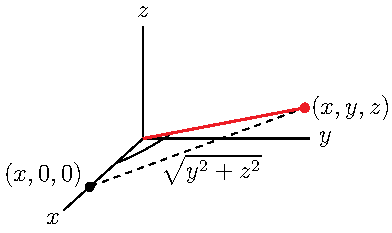
\includegraphics{sphericalX.pdf}
     \end{center}

}
we see that $\frac{\sqrt{y^2 + z^2}}{x}$ is the tangent of the
angle between the radius vector $(x,y,z)$ and the $x$-axis. The 
angle between the radius vector $(x,y,z)$ and the $z$-axis (not the $x$-axis)
is exactly spherical coordinate $\varphi$. So let's modify spherical
coordinates to make the $x$-axis play the role of the $z$-axis. 
The easy way to do is to just rename $x=Z$, $y=X$, $z=Y$. Then the integral
we are to compute becomes $\dblInt_S ZX^2\ \dee{S}$, and the
condition $x \ge \sqrt{y^2 + z^2}$ becomes $Z \ge \sqrt{X^2 + Y^2}$.
Under the parametrization 
\begin{align*}
X=\sqrt{2}\,\sin\varphi\cos\theta \qquad
Y=\sqrt{2}\,\sin\varphi\sin\theta \qquad
Z=\sqrt{2}\,\cos\varphi
\end{align*}
the condition $Z \ge \sqrt{X^2 + Y^2}$ is
$\frac{\sqrt{X^2 + Y^2}}{Z}=\frac{\sin\varphi}{\cos\varphi}\le 1$,
which is turn is $0\le\varphi\le\frac{\pi}{4}$. As
$\dee{S}=2\sin\varphi\,\dee{\theta}\dee{\varphi}$ 
(see Appendix \eref{CLP317}{ap:spherCoord} in the CLP-4 text and recall that $\rho=\sqrt{2}$) the specified integral
is
\begin{align*}
\dblInt_S xy^2\ \dee{S}
&=\dblInt_S ZX^2\ \dee{S}
=2\int_0^{\pi/4}\dee{\varphi}\ \sin\varphi \int_0^{2\pi}\dee{\theta}\ 
\big(\sqrt{2}\,\cos\varphi\big)\big(\sqrt{2}\,\sin\varphi\cos\theta\big)^2
\\
&=4\sqrt{2} \left\{\int_0^{\pi/4}\dee{\varphi}\ \cos\varphi\sin^3\varphi\right\}
            \left\{\int_0^{2\pi}\dee{\theta}\, \cos^2\theta\right\} \\
&=4\sqrt{2} \left\{\int_0^{\pi/4}\dee{\varphi}\ \cos\varphi\sin^3\varphi\right\}
           \left\{\int_0^{2\pi}\dee{\theta}\,\frac{\cos(2\theta)+1}{2}\right\} \\
&=4\sqrt{2} \left[\frac{\sin^4\varphi}{4}\right]_0^{\pi/4} 
     \left[\frac{\sin(2\theta)}{4}+\frac{\theta}{2}\right]_0^{2\pi} \\
&= \frac{\sqrt{2}\,\pi}{4}
\end{align*}
For an efficient, sneaky, way to evaluate 
$\int_0^{2\pi} \cos^2 \theta\ \dee{\theta}$, see Example
\eref{CLP317}{eg:workIntegalB} in the CLP-4 text.
\end{solution}

%%%%%%%%%%%%%%%%%%%%%%%%%%%%
\begin{question}[M317 2006D, 2012J] %2006D #3 and 2012J #6
Let $S$ be the surface given by the equation
\begin{align*}
x^2 + z^2 = \sin^2y
\end{align*}
lying between the planes $y = 0$ and $y = \pi$. Evaluate the integral
\begin{align*}
\dblInt_S\sqrt{1 + \cos^2y}\, \dee{S}
\end{align*}
\end{question}

\begin{hint} 
The surface $S$ may be parametrized by observing that, for each fixed 
$y$, $x^2 + z^2 = \sin^2y$ is a circle.
\end{hint}

\begin{answer} 
$\frac{16}{3}\pi$
\end{answer}

\begin{solution}
Here is a sketch of the part of $S$ that is in the first octant.

\begin{center}
       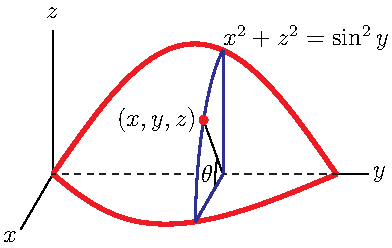
\includegraphics{OE06D_3.pdf}
\end{center}

For each fixed $y$, $x^2+z^2=\sin^2y$ is a circle of
radius $\sin y$. (It's the blue circle in the sketch above.)
So we may parametrize the surface by
\begin{align*}
\vr(\theta,y)
=\big(\sin y\,\cos\theta\,,\, y \,,\, \sin y\,\sin\theta\big)\qquad
0\le\theta<2\pi,\ 0\le y\le \pi
\end{align*}
Then, by (\eref{CLP317}{eq:SUdSparam}) in the CLP-4 text,
\begin{align*}
\frac{\partial \vr}{\partial\theta}
 &= \big(-\sin y\,\sin\theta\,,\, 0 \,,\, \sin y\,\cos\theta\big) \\
\frac{\partial \vr}{\partial y}
 &= \big(\cos y\,\cos\theta\,,\, 1 \,,\, \cos y\,\sin\theta\big) \\
\frac{\partial \vr}{\partial\theta} \times
     \frac{\partial \vr}{\partial y}
&=\big(-\sin y\,\cos\theta\,,\, \sin y\,\cos y\,,\,-\sin y\,\sin\theta \big) \\
\dee{S}
&= \left|\frac{\partial \vr}{\partial\theta} \times
     \frac{\partial \vr}{\partial y}\right|\dee{\theta}\,\dee{y}
=\sin y\sqrt{1+\cos^2 y}\ \dee{\theta}\ \dee{y}
\end{align*}
So the specified integral is
\begin{align*}
\dblInt_S\sqrt{1 + \cos^2y}\, \dee{S}
&= \int_0^\pi\dee{y} \int_0^{2\pi}\dee{\theta}\ 
                \sin y\big\{1+\cos^2 y\big\} \\
&= 2\pi \int_0^\pi\dee{y}\ 
                \sin y\big\{1+\cos^2 y\big\} \\
&= - 2\pi \int_1^{-1} \dee{u}\ \big\{1+u^2\big\}
           \quad\text{with }u=\cos y,\ \dee{u}=-\sin y\,\dee{y} \\
&= 4\pi \int_0^1 \dee{u}\ \big\{1+u^2\big\} \\
&=4\pi\left[u+\frac{u^3}{3}\right]_0^1 \\
&= \frac{16}{3}\pi
\end{align*}


\end{solution}

%%%%%%%%%%%%%%%%%%%%%%%%%%%
\begin{question}[M317 2006A] %5
Let $S$ be the part of the paraboloid $z=1-x^2-y^2$ lying above the 
$xy$-plane. At $(x,y,z)$ $S$ has density
\begin{align*}
\rho(x,y,z) = \frac{z}{\sqrt{5-4z}}
\end{align*} 
Find the centre of mass of $S$.
\end{question}

\begin{hint} 
By symmetry, the centre of mass will lie on the $z$-axis.
By definition, the $z$-coordinate of the centre of mass is the weighted
average of $z$ over $S$, which is
\begin{equation*}
\bar z = \frac{\dblInt_S z\,\rho(x,y,z)\ \dee{S}}
              {\dblInt_S \rho(x,y,z)\ \dee{S}}
\end{equation*}
\end{hint}

\begin{answer} 
$\big(0,0,\nicefrac{2}{3}\big)$
\end{answer}

\begin{solution}
The paraboloid is
\begin{equation*}
S = \Set{(x,y,z)}{z=1-x^2-y^2,\ z\ge 0}
  = \Set{(x,y,z)}{z=1-x^2-y^2,\ x^2+y^2\le 1}
\end{equation*}
By (\eref{CLP317}{eq:SUdSgraph}) in the CLP-4 text, the paraboloid has
\begin{align*}
\dee{S} & = \sqrt{1+f_x(x,y)^2 + f_y(x,y)^2}\,\dee{x}\dee{y}
\qquad\text{with } z = f(x,y) = 1-x^2-y^2 \\
        & = \sqrt{1+4x^2 +4y^2}\,\dee{x}\dee{y}
\end{align*}
By symmetry, the centre of mass will lie on the $z$-axis.
By definition, the $z$-coordinate of the centre of mass is the weighted
average of $z$ over $S$, which is
\begin{equation*}
\bar z = \frac{\dblInt_S z\,\rho(x,y,z)\ \dee{S}}
              {\dblInt_S \rho(x,y,z)\ \dee{S}}
\end{equation*}
On $S$,
\begin{align*}
\rho(x,y,z) = \frac{z}{\sqrt{5-4z}}
            = \frac{1-x^2-y^2}{\sqrt{1+4x^2+4y^2}}
\end{align*}
so that
\begin{align*}
\rho(x,y,z)\ \dee{S}
= (1-x^2-y^2)\,\dee{x}\dee{y}
\end{align*}
So, using polar coordinates, the denominator of $\bar z$ is
\begin{align*}
\dblInt_S \rho(x,y,z)\ \dee{S}
     &= \dblInt_{x^2+y^2\le 1} (1-x^2-y^2)\,\dee{x}\dee{y}
     =\int_0^1\dee{r}\, r\int_0^{2\pi}\dee{\theta}\,  (1-r^2) \\
    &= 2\pi\int_0^1 r(1-r^2)\ \dee{r} \\
    & = 2\pi \Big[\frac{r^2}{2}-\frac{r^4}{4}\Big]_0^1 \\
    &=\frac{\pi}{2}
\end{align*}
and the numerator of $\bar z$ is
\begin{align*}
\dblInt_S z \rho(x,y,z)\ \dee{S}
     &= \dblInt_{x^2+y^2\le 1} {(1-x^2-y^2)}^2\,\dee{x}\dee{y}
     =\int_0^1\dee{r}\, r\int_0^{2\pi}\dee{\theta}\,  {(1-r^2)}^2 \\
    &= 2\pi\int_0^1 r{(1-r^2)}^2\ \dee{r} \\
    & = 2\pi \Big[\frac{r^2}{2}-2\frac{r^4}{4}+\frac{r^6}{6}\Big]_0^1 \\
    &=\frac{\pi}{3}
\end{align*}
and
\begin{equation*}
\bar z = \frac{\pi/3}{\pi/2}=\frac{2}{3}
\end{equation*}
\end{solution}

%%%%%%%%%%%%%%%%%%%%%%%%%%%
\begin{question}[M317 2005D] %6
Let $S$ be the part of the plane
\begin{equation*}
x + y + z =2
\end{equation*}
that lies in the first octant oriented so that $\hn$ has a positive 
$\hk$ component. Let
\begin{equation*}
\vF = x\,\hi + y\,\hj + z\,\hk
\end{equation*}
Evaluate the flux integral
\begin{equation*}
\dblInt_S \vF\cdot\hn\, \dee{S}
\end{equation*}
\end{question}

%\begin{hint} 
%
%\end{hint}

\begin{answer} 
$4$
\end{answer}

\begin{solution}
The equation of the plane is $z=f(x,y) = 2-x-y$. So by
(\eref{CLP317}{eq:SUdSgraph}) in the CLP-4 text,
\begin{equation*}
\hn\,\dee{S} = \big[-f_x(x,y)\,\hi - f_y(x,y)\,\hj + \hk\big]\ \dee{x}\dee{y}
             = \big[\hi + \hj + \hk\big]\ \dee{x}\dee{y}
\end{equation*}
A point $(x,y,z)$ on the plane lies in the first octant if and only if
\begin{equation*}
x\ge 0\quad\text{and}\quad
y\ge 0\quad\text{and}\quad
z=2-x-y\ge 0
\end{equation*}
So the domain of integration is the triangle
\begin{equation*}
\hskip1.25in T = \Set{(x,y)}{x\ge 0,\ y\ge 0,\ x+y\le 2} \hskip0.75in
\raisebox{-25pt}[0pt][5pt]{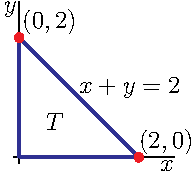
\includegraphics{OE05D_6.pdf}}
\end{equation*}
and
\begin{align*}
\dblInt_S \vF\cdot\hn\, \dee{S}
&=\dblInt_T \big[x\,\hi+y\,\hj +(\overbrace{2-x-y}^{z})\,\hk\big]
         \cdot\big[\hi + \hj + \hk\big]\ \dee{x}\dee{y} \\
& = 2 \dblInt_T \dee{x}\dee{y} \\
& = 2 \frac{1}{2}(2)(2) = 4
\end{align*}

\end{solution}

%%%%%%%%%%%%%%%%%%%%%%%%%%%
\begin{question}[M317 2005A] %4
Find the net flux $\dblInt_S \vF\cdot\hn\,\dee{S}$ of the vector field
$\vF(x,y,z) = (x,y,z)$ upwards (with respect to the $z$-axis) through
the surface $S$ parametrized $\vr = \big(uv^2\,,\,u^2v\,,\,uv\big)$
for $0\le u\le 1$, $0\le v\le 3$.
\end{question}

%\begin{hint} 
%
%\end{hint}

\begin{answer} 
$\frac{81}{16}$
\end{answer}

\begin{solution} Since
\begin{align*}
\tfrac{\partial\vr}{\partial u}
&=\big(v^2\,,\,
       2uv\,,\,
        v \big) \\
\tfrac{\partial\vr}{\partial v}
&=\big(2uv\,,\,
        u^2\,,\,
        u \big) \\
\tfrac{\partial\vr}{\partial u} \times \tfrac{\partial\vr}{\partial v} 
&=\big(u^2v\,,\,
       uv^2\,,\,
       -3u^2v^2\big)
\end{align*}
(\eref{CLP317}{eq:SUdSparam}) in the CLP-4 text gives
\begin{equation*}
\hn\,\dee{S} = \pm  \big(u^2v\,,\,
       uv^2\,,\,
       -3u^2v^2\big)\,\dee{u}\dee{v}
\end{equation*}
We are told that $\hn$ should have a positive $z$-component, so
\begin{equation*}
\hn\,\dee{S} = -  \big(u^2v\,,\, uv^2\,,\, -3u^2v^2\big)\,\dee{u}\dee{v}
 = \big(-u^2v\,,\, -uv^2\,,\, 3u^2v^2\big)\,\dee{u}\dee{v}
\end{equation*}
and
\begin{align*}
\dblInt_S \vF\cdot\hn\,\dee{S}
&=\dblInt_S \overbrace{(uv^2\,,\,u^2v\,,\,uv)}^{\vF}\cdot
         \big(-u^2v\,,\, -uv^2\,,\, 3u^2v^2\big)\,\dee{u}\dee{v} \\
&=\int_0^1\dee{u}\int_0^3\dee{v}\ u^3v^3 
=\left[\int_0^1\dee{u}\ u^3 \right]\  \left[\int_0^3\dee{v}\ v^3\right] \\
&=\frac{1}{4}\ \frac{3^4}{4}
=\frac{81}{16}
\end{align*} 
\end{solution}

\begin{question}[M317 2015A]  %2
Let $S$ be the surface obtained by revolving the curve 
$z = e^y$ , $0 \le y \le 1$, around the $y$-axis, with the 
orientation of $S$ having $\hn$ pointing toward the $y$-axis.
\begin{enumerate}[(a)]
\item
Draw a picture of $S$ and find a parameterization of $S$.

\item
Compute the integral $\dblInt_S e^y\, \dee{S}$.

\item
Compute the flux integral $\dblInt_S\vF\cdot\hn\,\dee{S}$
where $\vF= (x, 0, z)$.

\end{enumerate}
\end{question}

%\begin{hint} 
%\end{hint}

\begin{answer} 
(a) $
\vr(Y,\theta) = e^Y\sin\theta\,\hi + Y\,\hj +e^Y\cos\theta\,\hk\qquad
0\le Y\le 1,\ 0\le\theta\le 2\pi
$

\begin{center}
    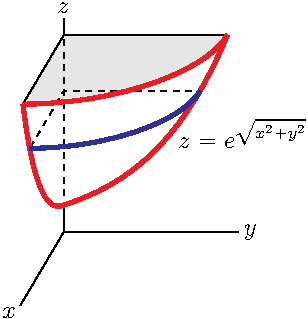
\includegraphics{revB.pdf}
\end{center}

(b) $\frac{2\pi}{3}\Big[(1+e^2)^{3/2}-2^{3/2}\Big]$\qquad
(c) $\pi\big(1-e^2\big)$
\end{answer}

\begin{solution} (a)
We start by just sketching the curve $z=e^y$, considering the $yz$-plane as 
the plane $x=0$ in $\bbbr^3$. This curve is the red curve 
in the figure below.
Concentrate on any one point on that curve. It is the blue dot at $(0,Y,e^Y)$
\vadjust{
\begin{center}
    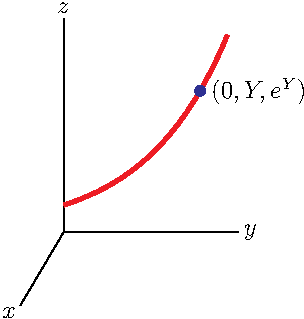
\includegraphics{revA.pdf}
\end{center}
}
in the figure. When our curve is rotated about the $y$-axis, the blue dot
sweeps out a circle. The circle that the blue dot sweeps out
\begin{itemize}\itemsep1pt \parskip0pt \parsep0pt %\itemindent-15pt
\item[$\circ$]
lies in the vertical plane $y=Y$ and
\item[$\circ$]
is centred on the $y$-axis and
\item[$\circ$]
has radius $e^Y$.
\end{itemize}
We can parametrize the circle swept out in the usual way. Here
is an end view of the circle (looking down the $y$-axis), with 
the parameter, named $\theta$, indicated. 
\begin{center}
    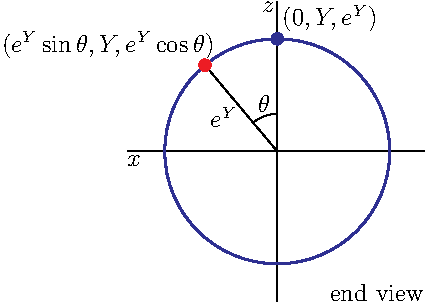
\includegraphics{revEnd.pdf}
\end{center}
The coordinates of the red dot are $\big(e^Y\sin\theta\,,\,Y\,,\,e^Y\cos\theta\big)$. This also gives 
a parametrization of the surface of revolution
\begin{align*}
x(Y,\theta) & = e^Y\sin\theta \\
y(Y,\theta) & = Y \\
z(Y,\theta) & = e^Y\cos\theta \\
&0\le Y\le 1,\qquad 0\le\theta<2\pi
\end{align*}
Finally here is a sketch of the part of the surface in the first octant,
$x,y,z\ge 0$.
\begin{center}
    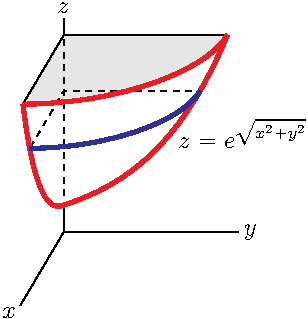
\includegraphics{revB.pdf}
\end{center}

(b) We are using the parametrization
\begin{equation*}
\vr(Y,\theta) = e^Y\sin\theta\,\hi + Y\,\hj +e^Y\cos\theta\,\hk\qquad
0\le Y\le 1,\ 0\le\theta\le 2\pi
\end{equation*}
so that
\begin{equation*}
\frac{\partial\vr}{\partial Y}\times\frac{\partial\vr}{\partial\theta}
= \det\left[\begin{matrix} \hi & \hj & \hk \\
e^Y\sin\theta & 1 & e^Y\cos\theta \\
e^Y\cos\theta & 0 & -e^Y\sin\theta \end{matrix}\right]
= \big(-e^Y\sin\theta, e^{2Y}, -e^Y\cos\theta\big),
\end{equation*}
and, by (\eref{CLP317}{eq:SUdSparam}) in the CLP-4 text,
\begin{align*}
\dee{S} = \Big|\frac{\partial\vr}{\partial Y}\times
            \frac{\partial\vr}{\partial\theta}\Big|\,\dee{Y}\dee{\theta}
= \sqrt{e^{2Y}+e^{4Y}}\,\dee{Y}\,\dee{\theta}
= e^Y\sqrt{1+e^{2Y}}\,\dee{Y}\dee{\theta}
\end{align*}
So the integral is
\begin{align*}
\dblInt_S e^y\, \dee{S}
&=\int_0^1\dee{Y}\int_0^{2\pi}\dee{\theta}\ e^{2Y}\sqrt{1+e^{2Y}}
=2\pi \int_0^1\dee{Y}\ e^{2Y}\sqrt{1+e^{2Y}}
=\frac{2\pi}{3}\Big[1+e^{2Y}\Big]^{3/2}\bigg|_0^1 \\
&=\frac{2\pi}{3}\Big[(1+e^2)^{3/2}-2^{3/2}\Big]
\end{align*}

(c) Again, we are using the parametrization
\begin{equation*}
\vr(Y,\theta) = e^Y\sin\theta\,\hi + Y\,\hj +e^Y\cos\theta\,\hk\qquad
0\le Y\le 1,\ 0\le\theta\le 2\pi
\end{equation*}
so that
\begin{equation*}
\frac{\partial\vr}{\partial Y}\times\frac{\partial\vr}{\partial\theta}
= \big(-e^Y\sin\theta, e^{2Y}, -e^Y\cos\theta\big),
\end{equation*}
and, by (\eref{CLP317}{eq:SUdSparam}) in the CLP-4 text,
\begin{align*}
\hn\,\dee{S} = \pm\frac{\partial\vr}{\partial Y}\times
            \frac{\partial\vr}{\partial\theta}\,\dee{Y}\dee{\theta}
= \pm\big(-e^Y\sin\theta, e^{2Y}, -e^Y\cos\theta\big)\,\dee{Y}\,\dee{\theta}
\end{align*}
We choose the ``$+$'' sign so that $\hn$ points towards the $y$-axis.
As an example, when $0\le\theta\le\frac{\pi}{2}$, then $z=e^Y\cos\theta>0$
while the $z$-coordinate of $\hn$ is $-e^y\cos\theta<0$. So the integral is
\begin{align*}
\dblInt_S\vF\cdot\hn\,\dee{S}
&=\int_0^1\dee{Y}\int_0^{2\pi}\dee{\theta}\ 
\big(\overbrace{e^Y\sin\theta}^{x},0,\overbrace{e^Y\cos\theta}^{z}\big)
           \cdot\big(-e^Y\sin\theta, e^{2Y}, -e^Y\cos\theta\big) \\
&=-\int_0^1\dee{Y}\int_0^{2\pi}\dee{\theta}\ e^{2Y}
=-2\pi\int_0^1\dee{Y}\ e^{2Y} \\
&=-\pi\big(e^2-1\big)
=\pi\big(1-e^2\big)
\end{align*}
\end{solution}

%%%%%%%%%%%%%%%%%%%%%%%%%%%%%%%
\begin{question}[M317 2011A] %5
Compute the net outward flux of the vector field
\begin{equation*}
\vF = \frac{\vr}{|\vr|}
    = \frac{x\,\hi+y\,\hj+z\,\hk}{\sqrt{x^2+y^2+z^2}}
\end{equation*}
across the boundary of the region \emph{between} the spheres of 
radius $1$ and radius $2$ centred at the origin.
\end{question}

%\begin{hint} 
%
%\end{hint}

\begin{answer} 
$12\pi$
\end{answer}

\begin{solution} 
Write
\begin{equation*}
V=\Set{(x,y,z)}{ 1\le x^2+y^2+z^2\le 4}
\end{equation*}
The boundary of $V$ consists of two parts ---
the sphere, $S_2$, of radius $2$, centred on the origin,
with (outward) normal $\hn=\frac{\vr}{|\vr|}=\frac{\vr}{2}$,
and the sphere  $S_1$ of radius $1$, centred on the origin,
with (inward) normal $\hn = -\vr$, So,
\begin{align*}
\dblInt_{\partial V} \vF\cdot\hn\,\dee{S}
&=\dblInt_{S_2} \frac{\vr}{|\vr|}\cdot\frac{\vr}{2}\,\dee{S}
-\dblInt_{S_1} \frac{\vr}{|\vr|}\cdot\vr\,\dee{S} \\
&=\dblInt_{S_2} \dee{S}
   -\dblInt_{S_1} \dee{S} \\
&=4\pi(2)^2 -4\pi(1)^2 \\
&=12\pi
\end{align*} 
\end{solution}

%%%%%%%%%%%%%%%%%%%%%%%%%%%%%%%%
%\begin{question}[M317 2012J] %6
%Let $S$ be the surface given by the equation
%\begin{equation*}
%x^2 + z^2 = \sin^2 y
%\end{equation*}
%lying between the planes $y = 0$ and $y = \pi$.
%\begin{enumerate}[(a)]
%\item
%Draw a picture of the surface $S$ in $\bbbr^3$ including the coordinate axes.
%\item
%Find a parameterization of $S$.
%\item
%Evaluate the integral
%\begin{equation*}
%\dblInt_S\sqrt{1+\cos^2(y)}\,\dee{S}
%\end{equation*}
%\end{enumerate}
%
%\end{question}
%
%\begin{hint} 
%First consider the constant $y$ cross-sections of $S$.
%\end{hint}
%
%\begin{answer} 
%$\frac{16\pi}{3}$
%\end{answer}
%
%\begin{solution} 
%(a), (b) For each fixed $0\le Y\le \pi$, the cross-section
%of $S$ with $y=Y$ is the circle $x^2+z^2 = \sin^2 Y$, $y=Y$. The radius of
%this circle, $\sin Y$, is $0$ for $Y=0$ and $Y=\pi$  and is (a maximum of) $1$
%when $Y=\frac{\pi}{2}$.  Here is a sketch of the part of $S$ that is in
%the first octant.
%\begin{center}
%     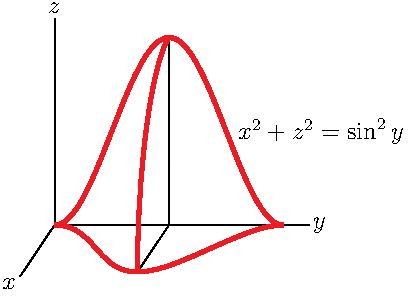
\includegraphics[scale=0.90]{OE12J_6.pdf}
%\end{center}
%We can parametrize the circle in the usual way
%\begin{align*}
%x(Y,\theta) &=\sin Y\,\cos\theta \\
%z(Y,\theta) &=\sin Y\,\sin\theta \\
%y(Y,\theta) &=Y
%\end{align*}
%This also gives a parametrization of $S$
%\begin{align*}
%\vr(Y,\theta) = \sin Y\,\cos\theta\,\hi +Y\,\hj + \sin Y\,\sin\theta\,\hk
%\qquad
%0\le Y\le\pi,\ 0\le\theta\le 2\pi
%\end{align*}
%
%(c)
%As
%\begin{equation*}
%\frac{\partial\vr}{\partial Y}\times\frac{\partial\vr}{\partial\theta}
%= \det\left[\begin{matrix} \hi & \hj & \hk \\
%\cos Y\cos\theta & 1 & \cos Y\sin\theta \\
%-\sin Y\sin\theta & 0 & \sin Y\cos\theta \end{matrix}\right]
%= \big(\sin Y\cos\theta, -\sin Y\cos Y, \sin Y\sin\theta\big),
%\end{equation*}
%and, by (\eref{CLP317}{eq:SUdSparam}) in the CLP-4 text,
%\begin{align*}
%\dee{S} &= \Big|\frac{\partial\vr}{\partial Y}\times
%            \frac{\partial\vr}{\partial\theta}\Big|\,\dee{Y}\dee{\theta}
%= \sqrt{\sin^2Y\cos^2\theta + \sin^2 Y\cos^2 Y 
%                + \sin^2Y\sin^2\theta}\,\dee{Y}\,\dee{\theta} \\
%&= \sin Y\sqrt{1+\cos^2 Y}\,\dee{Y}\dee{\theta}
%\end{align*}
%the integral is
%\begin{align*}
%\dblInt_S\sqrt{1+\cos^2(y)}\,\dee{S}
%&=\int_0^\pi\dee{Y}\int_0^{2\pi}\dee{\theta}\ \sin Y \big(1+\cos^2 Y\big)
%=2\pi \int_0^\pi\dee{Y}\ \sin Y \big(1+\cos^2 Y\big) \\
%&=- 2\pi \int_1^{-1} \big(1+u^2\big)\,\dee{u}
%\qquad\text{with } u = \cos Y,\ \dee{u}=-\sin Y\,\dee{Y} \\
%&= 4\pi\int_0^1 \big(1+u^2\big)\,\dee{u}
%=4\pi\Big(1+\frac{1}{3}\Big) \\
%&=\frac{16\pi}{3}
%\end{align*}
%\end{solution}

%%%%%%%%%%%%%%%%%%%%%%%%%%%%%%%
\begin{question}[M317 2016D] %7
Evaluate the surface integral $\dblInt_S z^2\,\dee{S}$ where $S$ is the 
part of the cone $x^2+y^2=4z^2$ where $0 \le x \le y$ and $0 \le z \le 1$.
\end{question}

%\begin{hint} 
%
%\end{hint}

\begin{answer} 
$\frac{\sqrt{5}\ \pi}{8}$
\end{answer}

\begin{solution} 
The part of the cone that has some fixed value, $Z$, of $z$ with $0\le Z\le 1$
is the part of the circle $\Set{(x,y,z)}{x^2+y^2=4Z^2, z=Z}$ of radius $2Z$
that has $0\le x\le y$. Here is a sketch of the top view of that part of that 
circle.
\begin{center}
     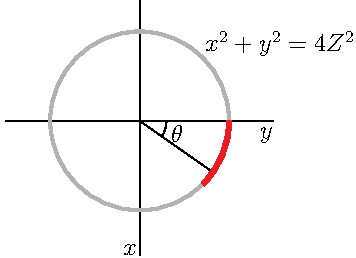
\includegraphics[scale=0.90]{OE16D_7.pdf}
\end{center}
So we can parametrize $S$ by
\begin{equation*}
\vr(\theta,Z) = 2Z\sin\theta\,\hi +2Z\cos\theta\,\hj + Z\,\hk\qquad
0\le\theta\le\frac{\pi}{4},\ 0\le Z\le 1
\end{equation*}
So
\begin{align*}
\frac{\partial\vr}{\partial\theta}
&= 2Z\cos\theta\,\hi -2Z\sin\theta\,\hj  \\
\frac{\partial\vr}{\partial Z}
&= 2\sin\theta\,\hi +2\cos\theta\,\hj + \hk
\end{align*}
so that
\begin{equation*}
\frac{\partial\vr}{\partial\theta}\times\frac{\partial\vr}{\partial Z}
= \det\left[\begin{matrix} \hi & \hj & \hk \\
2Z\cos\theta & -2Z\sin\theta & 0 \\
2\sin\theta & 2\cos\theta & 1\end{matrix}\right]
= \big(-2Z\sin\theta, -2Z\cos\theta, 4Z\big),
\end{equation*}
and, by (\eref{CLP317}{eq:SUdSparam}) in the CLP-4 text,
\begin{align*}
\dee{S} = \left|\frac{\partial\vr}{\partial\theta}\times
            \frac{\partial\vr}{\partial Z}\right|\,\dee{\theta}\dee{Z}
= \sqrt{20}\,Z\,\dee{\theta}\dee{Z}
\end{align*}
and
\begin{align*}
\dblInt_S z^2\,\dee{S}
&=\sqrt{20} \int_0^1\dee{Z}\int_0^{\pi/4}\dee{\theta}\ Z^3
=\sqrt{20}\ \frac{\pi}{4}\ \frac{1}{4}
=\frac{\sqrt{5}\ \pi}{8}
\end{align*}
\end{solution}

%%%%%%%%%%%%%%%%%%%%%%%%%%%
\begin{question}[M317 2017A] %4
Compute the flux integral $\dblInt_S \vF\cdot\hn\,\dee{S}$, where
\begin{equation*}
\vF = \Big(-\frac{1}{2}x^3 - xy^2 \,,\, -\frac{1}{2} y^3 \,,\, z^2\Big)
\end{equation*}
and $S$ is the part of the paraboloid $z = 5 - x^2 - y^2$ 
lying inside the cylinder $x^2 + y^2 \le 4$,
with orientation pointing downwards.
\end{question}

%\begin{hint} 
%\end{hint}

\begin{answer} 
$-20\,\pi$
\end{answer}

\begin{solution} 
We'll start by parametrizing $S$. Note that as $x^2+y^2$
runs from $0$ to $4$, $z$ runs from $5$ to $1$, and that, for each
fixed $1\le Z\le 5$, the cross-section of $S$ with $z=Z$
is the circle $x^2+y^2=5-Z$, $z=Z$. So we may parametrize $S$ by
\begin{equation*}
\vr(\theta, Z) = \sqrt{5-Z}\cos\theta\,\hi
                +\sqrt{5-Z}\sin\theta\,\hj
                +Z\,\hk\qquad
0\le\theta\le 2\pi,\ 1\le Z\le 5
\end{equation*}
Since
\begin{align*}
\frac{\partial\vr}{\partial\theta}
&= -\sqrt{5-Z}\sin\theta\,\hi +\sqrt{5-Z}\cos\theta\,\hj  \\
\frac{\partial\vr}{\partial Z}
&= -\frac{1}{2\sqrt{5-Z}}\cos\theta\,\hi -\frac{1}{2\sqrt{5-Z}}\sin\theta\,\hj 
  + \hk
\end{align*}
so that
\begin{equation*}
\frac{\partial\vr}{\partial\theta}\times\frac{\partial\vr}{\partial Z}
= \det\left[\begin{matrix} \hi & \hj & \hk \\[0.05in]
-\sqrt{5-Z}\sin\theta & \sqrt{5-Z}\cos\theta & 0 \\[0.05in]
-\frac{1}{2\sqrt{5-Z}}\cos\theta &-\frac{1}{2\sqrt{5-Z}}\sin\theta & 1
         \end{matrix}\right]
= \big(\sqrt{5-Z}\cos\theta\,,\,\sqrt{5-Z}\sin\theta\,,\, 1/2\big),
\end{equation*}
(\eref{CLP317}{eq:SUdSparam}) in the CLP-4 text gives
\begin{align*}
\hn\,\dee{S} = \pm \frac{\partial\vr}{\partial\theta}\times
            \frac{\partial\vr}{\partial Z}\,\dee{\theta}\dee{Z}
= \pm \big(\sqrt{5-Z}\cos\theta\,,\,\sqrt{5-Z}\sin\theta\,,\, 1/2\big)
          \,\dee{\theta}\dee{Z}
\end{align*}
Choosing the minus sign to give the downward pointing normal
\begin{align*}
&\dblInt_S \vF\cdot\hn\,\dee{S}\\
&=-\int_1^5\hskip-3pt\dee{Z}\int_0^{2\pi}\hskip-6.5pt\dee{\theta}\ 
    \Big(-\frac{1}{2}\overbrace{[5-Z]^{3/2}\cos^3\theta}^{x^3} 
           - \overbrace{[5-Z]^{3/2}\cos\theta\sin^2\theta}^{xy^2} \,,\, 
         -\frac{1}{2}\overbrace{[5-Z]^{3/2}\sin^3\theta}^{y^3} \,,\, 
         \overbrace{Z^2}^{z^2}\Big) \\
&\hskip4in \cdot
    \big(\sqrt{5-Z}\cos\theta\,,\,\sqrt{5-Z}\sin\theta\,,\, 1/2\big) \\
&=-\int_1^5\hskip-3pt\dee{Z}\int_0^{2\pi}\hskip-6.5pt\dee{\theta}\ 
    \Big(-\frac{1}{2}[5-Z]^2\cos^4\theta
           - [5-Z]^2\cos^2\theta\sin^2\theta 
         -\frac{1}{2}[5-Z]^2\sin^4\theta  
         +\frac{1}{2}Z^2\Big)
\end{align*}
Since 
\begin{equation*}
\frac{1}{2}\cos^4\theta + \cos^2\theta\sin^2\theta +\frac{1}{2}\sin^4\theta 
=\frac{1}{2}\big(\cos^2\theta+\sin^2\theta\big)^2=\frac{1}{2}
\end{equation*}
the flux
\begin{align*}
\dblInt_S \vF\cdot\hn\,\dee{S}
&=\int_1^5\hskip-3pt\dee{Z}\int_0^{2\pi}\hskip-6.5pt\dee{\theta}\ 
    \Big(\frac{1}{2}[5-Z]^2 -\frac{1}{2} Z^2\Big)
=\pi \int_1^5\hskip-3pt\dee{Z}\ \Big([5-Z]^2 -Z^2\Big) \\
&=\pi\left[-\frac{1}{3}[5-Z]^3 - \frac{Z^3}{3}\right]_1^5
=\pi \left[\frac{4^3}{3}-\frac{5^3}{3}+\frac{1}{3}\right]
=-20\,\pi
\end{align*}
\end{solution}


%%%%%%%%%%%%%%%%%%%%%%%%%%%
\begin{question}[M317 2003A] %4
Let the thin shell $S$ consist of the part of the surface $z^2=2xy$
with $x\ge 1$, $y\ge 1$ and $z\le 2$. Find the mass of $S$ if it has surface
density given by $\rho(x,y,z)=3z$ kg per unit area.
\end{question}

%\begin{hint} 
%\end{hint}

\begin{answer} 
$3$
\end{answer}

\begin{solution} 
The surface is $z=f(x,y)$ with $f(x,y)=\sqrt{2xy}$. Since
$f_x=\sqrt{\frac{y}{2x}}$ and $f_y=\sqrt{\frac{x}{2y}}$,
(\eref{CLP317}{eq:SUdSgraph}) in the CLP-4 text gives
\begin{align*}
\dee{S}&=\sqrt{1+f_x^2+f_y^2}\,\dee{x}\dee{y}
=\sqrt{1+\frac{y}{2x}+\frac{x}{2y}}\,\dee{x}\dee{y}
=\sqrt{\frac{2xy+y^2+x^2}{2xy}}\,\dee{x}\dee{y} \\
&=\frac{x+y}{\sqrt{2xy}}\,\dee{x}\dee{y}
\end{align*}
On the shell, $z^2=2xy\le 4$. So the $x$ and $y$ components of 
points $(x,y,z)$ on the shell run over the region $x\ge 1$, $y\ge 1$, 
$xy\le 2$, which
is sketched below
\begin{center}
     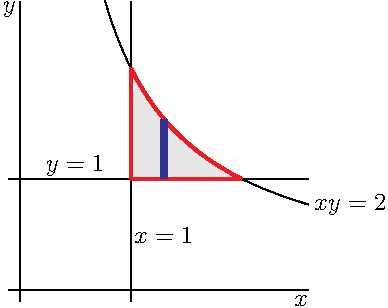
\includegraphics{OE03A_4.pdf}
\end{center}
So the mass is
\begin{align*}
\dblInt_S \rho(x,y,z)\,dS
&=\int_1^2\dee{x}\int_1^{2/x}\dee{y}\ 3f(x,y)\frac{x+y}{\sqrt{2xy}}
=\int_1^2\dee{x}\int_1^{2/x}\dee{y}\ 3(x+y) \\
&=3\int_1^2\dee{x}\ \left[xy+\frac{1}{2} y^2\right]_1^{2/x}
=3\int_1^2 \dee{x}\ \left[2+\frac{2}{x^2}-x-\frac{1}{2}\right] \\
&=3\left\{\frac{3}{2}-\frac{2}{x}\bigg|_1^2-\frac{x^2}{2}\bigg|^2_1\right\}
=3\left\{\frac{3}{2}-1+2-2+\frac{1}{2}\right\} \\
&=3
\end{align*}
\end{solution}


%%%%%%%%%%%%%%%%%%%%%%%%%%%
\begin{question}[M317 2003A] %5
Let $S$ be the portion of the paraboloid $x=y^2 + z^2$ that satisfies
$x \le 2 y $. Its unit normal vector $\hn$ is so chosen that
$\hn \cdot \hi > 0$. Find the flux of 
$\vF =  2\,\hi +  z\,\hj + y\,\hk$ out of $S$.
\end{question}

%\begin{hint} 
%\end{hint}

\begin{answer} 
$2\pi$
\end{answer}

\begin{solution} 
Since $x=g(y,z)$ with $g(x,y)=y^2+z^2$, 
(\eref{CLP317}{eq:SUdSgraph}) in the CLP-4 text gives 
\begin{equation*}
\hn\,\dee{S}=\pm (1,-g_y,-g_z)\,\dee{y}\dee{z}
=\pm (1,-2y,-2z)\,\dee{y}\dee{z}
\end{equation*} 
We choose the $+$ sign so that $\hn \cdot \hi > 0$. Furthermore 
\begin{align*}
S&=\Set{(x,y,z)}{x=y^2+z^2,\ x\le 2y} \\
&=\Set{(x,y,z)}{x=y^2+z^2,\ y^2+z^2\le 2y} \\
&=\Set{(x,y,z)}{x=y^2+z^2,\ (y-1)^2+z^2\le 1} \\
&=\Set{(x,y,z)}{x=y^2+z^2,\ (y,z)\text{ in }D}
\end{align*}
where $D=\Set{(x,y)}{(y-1)^2+z^2\le 1}$ is a disk with radius $1$. Hence
$$
\dblInt_S \vF \cdot \hn\ \dee{S}
 = \dblInt_D (2, z, y) \cdot  (1,-2 y, -2z)\ \dee{y} \dee{z}
 = \dblInt_D (2 - 4yz)\ \dee{y} \dee{z}
$$
Since $-4yz$ is odd under $z\rightarrow -z$ the integral of $-4yz$ is zero and
\begin{equation*}
\dblInt_S \vF \cdot \hn\, \dee{S}= 2\,\text{Area}(D)=2\pi
\end{equation*}
\end{solution}


%%%%%%%%%%%%%%%%%%%%%%%%%%%
\begin{question}[M317 2001D] %5
Let $S$ denote the portion of the paraboloid 
$z=1-\frac{1}{4}x^2-y^2$ for which $z\ge 0$. Orient $S$ so that its unit
normal has a positive $\hat k$ component. Let
$$
\vF(x,y,z) = (3y^2+z)\,\hi+(x-x^2)\,\hj+\hk 
$$
Evaluate the surface integral $\dblInt_S\nabla\times\vF\cdot\hn\,\dee{S}$.
\end{question}

%\begin{hint} 
%\end{hint}

\begin{answer} 
$2\pi$
\end{answer}

\begin{solution} 
For the specified $\vF$ and the surface 
$x=f(x,y)=1-\frac{1}{4}x^2-y^2$, by (\eref{CLP317}{eq:SUdSgraph}) in the CLP-4 text,
\begin{align*}
\hn\,\dee{S}&=\big(-f_x\,\hi-f_y\,\hj+\hk\big)\,\dee{x}\dee{y}
=\Big(\frac{x}{2}\,\hi+2y\,\hj+\hk\Big)\,\dee{x}\dee{y}\\
\nabla\times\vF&=\det\left[\begin{matrix}\hi&\hj&\hk\\[0.03in] 
     \frac{\partial\hfill}{\partial x}&
        \frac{\partial\hfill}{\partial y}&
        \frac{\partial\hfill}{\partial z}\\[0.03in]
3y^2+z&x-x^2&1\end{matrix}\right] \\
&=\hj+(1-2x-6y)\,\hk\\
\nabla\times\vF\cdot\hn\,\dee{S}&= (2y+1-2x-6y)\,\dee{x}\dee{y}= (1-2x-4y)\,\dee{x}\dee{y}
\end{align*}
The domain of integration is $1-\frac{1}{4}x^2-y^2\ge 0$ or
$\frac{1}{4}x^2+y^2\le 1$. This is an ellipse. Call it $D$. 
So
$$
\dblInt_S\nabla\times\vF\cdot\hn\,\dee{S}
=\dblInt_D (1-2x-4y)\,\dee{x}\dee{y}
$$
The integrals over $D$ of $x$, which is odd under $x\rightarrow-x$, 
and of $y$, which is odd under $y\rightarrow -y$, are both zero.
As the ellipse $D$ has area $A=\pi\times 2\times 1=2\pi$ 
$$
\dblInt_S\nabla\times\vF\cdot\hn\,\dee{S}
=\dblInt_D (1-2x-4y)\,\dee{x}\dee{y}
=A
=2\pi
$$
\end{solution}

%%%%%%%%%%%%%%%%%%%%%%%%%%%
\begin{question} 
Let $S$ be the boundary of the apple core bounded by the sphere 
$x^2+y^2+z^2=16$ and the hyperboloid $x^2+y^2-z^2=8$.
Find the flux integral
$\ \dblInt_S\vF\cdot\hn \,dS\ $ where
$\vF=x\,\hi+y\,\hj+z\,\hk$
and $\hn$ is
the outward normal to the surface $S$.
\end{question}

\begin{hint}
You can use the the cylindrical coordinates $\theta$ and $z$ to 
parametrize the hyperboloid. 
\end{hint}

\begin{answer} 
$192\pi$
\end{answer}

\begin{solution} 
 Due to the symmetry of the surface and the vector field under reflection in the $xy$-plane, i.e. under $z\rightarrow -z$, it is sufficient
to compute the integral over the upper half of the surface, where $z \ge 0$,
and then multiply the result by 2. The upper half of the surface consists
of two pieces, $S_1$ and $S_2$, where $S_1$ is the part on the sphere and
$S_2$ is the part on the hyperboloid.
$S_1$ and $S_2$ intersect on a circle. The circle is obtained 
by imposing the two equations $x^2+y^2+z^2=16$ and $x^2+y^2-z^2=8$
simultaneously. Thus we have $x^2+y^2=12$ and $z=2$, or in cylindrical coordinates $r=\sqrt{12}$, $z=1$, on the circle. Here is a sketch of a 
cross-section of the apple core.
\begin{center}
    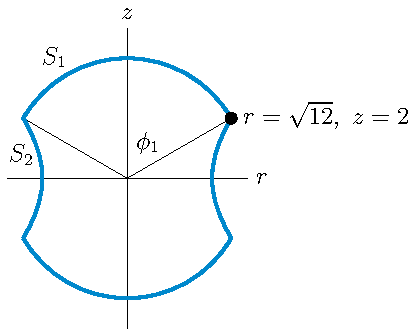
\includegraphics{applecore.pdf}
\end{center}
Let $\phi_1$ be the angle between $z$-axis and the cone formed by 
connecting the circle to the origin. We have $\tan \phi_1 = \sqrt {12}/2 = \sqrt 3$.  Thus $\phi_1 = \pi/3$.


We'll use spherical coordinates to compute the flux integral 
$\ \dblInt_{S_1}\vF\cdot\hn \,dS\ $. As the spherical coordinate
$\rho=4$ on all of $S_1$, we can paramerize $S_1$ by
\begin{align*}
\vr(\theta,\varphi) & = 4\cos\theta\sin\varphi \,\hi
                      + 4\sin\theta\sin\varphi \,\hj
                      + 4\cos\varphi \,\hk\qquad
0 \le \theta \le 2 \pi,\ 
0 \le \phi \le \pi/3
\end{align*}
So
\begin{align*}
\frac{\partial\vr}{\partial\theta}
&= -4\sin\theta\sin\varphi \,\hi
                      + 4\cos\theta\sin\varphi \,\hj \\
\frac{\partial\vr}{\partial\varphi}
&= 4\cos\theta\cos\varphi \,\hi
                      + 4\sin\theta\cos\varphi \,\hj
                      - 4\sin\varphi \,\hk \\
\frac{\partial\vr}{\partial\theta}\times\frac{\partial\vr}{\partial\varphi}
&= \det\left[\begin{matrix} \hi & \hj & \hk \\
-4\sin\theta\sin\varphi & 4\cos\theta\sin\varphi & 0 \\
4\cos\theta\cos\varphi & 4\sin\theta\cos\varphi & -4\sin\varphi 
             \end{matrix}\right] \\
&= -16\big(\cos\theta\sin^2\varphi\,,\, \sin\theta\sin^2\varphi\,,\,
                    \sin\varphi\cos\varphi\big) \\
&= -4\,(\sin\varphi)\,\vr(\theta,\varphi)
\end{align*}
and, by (\eref{CLP317}{eq:SUdSparam}) in the CLP-4 text,
\begin{align*}
\hn\,\dee{S} &= \pm\frac{\partial\vr}{\partial\theta}\times
            \frac{\partial\vr}{\partial\varphi}\,\dee{\theta}\dee{\varphi}
= \mp 4\,(\sin\varphi)\,\vr(\theta,\varphi)\,\dee{\theta}\dee{\varphi}  
\end{align*}
To get the outward pointing normal, i.e. the normal point in the same direction
as $\vr(\theta,\varphi)$, we take the plus sign. As $\vF = \vr(\theta,\varphi)$,
\begin{equation*}
\vF\cdot \hn\,\dee{S}
= 4\overbrace{|\vr(\theta,\varphi)|^2}^{4^2}\ \sin\varphi\,\dee{\theta}\,\dee{\varphi}
= 64 \sin\varphi\,\dee{\theta}\,\dee{\varphi}
\end{equation*}
and
\begin{align*}
\dblInt_{S_1}\vF\cdot\hn \,dS
= 64 \int_{0}^{2\pi} \dee{\theta} \int_{0}^{\pi/3}\dee{\varphi}\  \sin \varphi
= 64 \cdot 2\pi \Big[ - \cos \varphi \Big]_0^{\pi/3}
= 64 \pi
\end{align*}

The surface $S_2$ can be parametrized using the cylindrical coordinates
$\theta$ and $z$. Indeed, we have 
\begin{equation*}
r= \sqrt {x^2+y^2}= (8+z^2)^{1/2}
\end{equation*}
for the hyperboloid  and we always have $x=r \cos \theta$ and 
$y= r \sin \theta$. 
Thus the hyperboloid has the following parametrization:
\begin{align*}
\vR(\theta,z) = (8+z^2)^{1/2} \cos \theta \, \hi + 
(8+z^2)^{1/2} \sin \theta \, \hj + z \,\hk
\end{align*}
The range for the parameters of $S_2$ is $0 \le \theta \le 2\pi$ and 
$0  \le z \le 2$. We have
\begin{align*}
\pdiff{\vR}{\theta} &= -(8+z^2)^{1/2} \sin \theta \, \hi +
                   (8+z^2)^{1/2} \cos \theta \, \hj + 0 \,\hk\\
\pdiff{\vR}{z} &= z(8+z^2)^{-1/2} \cos \theta \, \hi 
        + z(8+z^2)^{-1/2} \sin \theta \, \hj +  \,\hk
\end{align*}
and
\begin{align*}
\pdiff{\vR}{\theta} \times \pdiff{\vR}{z} 
&=\det\left[\begin{matrix}\hi & \hj & \hk\\
             -(8+z^2)^{1/2} \sin \theta & (8+z^2)^{1/2} \cos \theta  & 0 \\
           z(8+z^2)^{-1/2} \cos \theta & z(8+z^2)^{-1/2} \sin \theta & 1
    \end{matrix}\right] \\[0.05in]
&= (8+z^2)^{1/2} \cos \theta \,\hi + (8+z^2)^{1/2} \sin\theta\,\hj - z \,\hk \\
&=x\,\hi + y\,\hj -z\,\hk
\end{align*}
Note that $\pdiff{\vR}{\theta} \times \pdiff{\vR}{z}$ is pointing 
downward (since $z>0$) and hence outward. 
Since $F \cdot \left(\pdiff{\vR}{\theta} \times \pdiff{\vR}{z} \right) 
= (x,y,z) \cdot (x,y,-z) =  x^2 + y^2 - z^2 = 8$ on $S_2$,
we have
\begin{equation*}
 \dblInt_{S_2}\vF\cdot\hn \,\dee{S}
=  \ \dblInt_{S_2} \vF \cdot (\vR_\theta \times \vR_z) \, d \theta\, \dee{z}   
=\int_0^2 \dee{z} \int_0^{2\pi}\dee{\theta}\ 8   
= 32 \pi
\end{equation*}
Finally, the flux integral over the whole apple core surface is  
\begin{equation*}
2  \left(\dblInt_{S_1}\vF\cdot\hn \,dS
+ \dblInt_{S_2}\vF\cdot\hn \,dS\right) 
= 2\big(64\pi+32\pi\big)
=192\pi
\end{equation*}
\end{solution}



%%%%%%%%%%%%%%%%%%
\subsection*{\Application}
%%%%%%%%%%%%%%%%%%

\begin{question}[M317 2012D] %5

\begin{enumerate}[(a)]
\item
Consider the surface $S$ given by the equation
\begin{equation*}
x^2 + z^2 = \cos^2 y 
\end{equation*}
Find an equation for the tangent plane to $S$ at the point 
$\big(\frac{1}{2} , \frac{\pi}{4} , \frac{1}{2} \big)$.
\item
Compute the integral
\begin{equation*}
\dblInt_S \sin y\ \dee{S}
\end{equation*}
where $S$ is the part of the surface from (a) lying between the planes 
$y = 0$ and $y = \frac{1}{2}\pi$.
\end{enumerate}
\end{question}

\begin{hint} 
(a)  Review \S\eref{CLP317}{sec:tangentPlanes} of the CLP-4 text.

(b)  Review \S\eref{CLP317}{subsec:paramSurfaces} of the CLP-4 text.
\end{hint}

\begin{answer} 
(a) $x+y+z = 1+\pi/4$\qquad
(b) $\frac{2\pi}{3}\big[2\sqrt{2}-1\big]$

\end{answer}

\begin{solution} (a)
The specified surface is of the form
\begin{equation*}
G(x,y,z) = x^2 + z^2 - \cos^2 y = 0
\end{equation*}
So one normal vector at the point 
       $\big(\frac{1}{2} , \frac{\pi}{4} , \frac{1}{2} \big)$
is
\begin{equation*}
\vnabla G\left(\frac{1}{2} , \frac{\pi}{4} , \frac{1}{2} \right)
=\big(2x \,,\, 2\sin y\cos y \,,\, 2z \big)\Big|_{
             \big(\frac{1}{2} , \frac{\pi}{4} , \frac{1}{2} )}
=(1,1,1)
\end{equation*}
and an equation for the tangent plane at 
   $\big(\frac{1}{2} , \frac{\pi}{4} , \frac{1}{2} \big)$
is
\begin{align*}
(1,1,1)\cdot\big(x-1/2\,,\,y-\pi/4\,,\, z-1/2\big) =0\quad\text{or}\quad
x+y+z = 1+\pi/4
\end{align*}

\noindent (b) For each fixed $y$, $x^2+z^2=\cos^2y$ is a circle of
radius $|\cos y|$. So we may parametrize the surface by
\begin{align*}
\vr(\theta,y)
=\big(\cos y\,\cos\theta\,,\, y \,,\, \cos y\,\sin\theta\big)\qquad
0\le\theta<2\pi,\ 0\le y\le \nicefrac{\pi}{2}
\end{align*}
Then
\begin{align*}
\frac{\partial \vr}{\partial\theta}
 &= \big(-\cos y\,\sin\theta\,,\, 0 \,,\, \cos y\,\cos\theta\big) \\
\frac{\partial \vr}{\partial y}
 &= \big(-\sin y\,\cos\theta\,,\, 1 \,,\, -\sin y\,\sin\theta\big) \\
\frac{\partial \vr}{\partial\theta} \times
     \frac{\partial \vr}{\partial y}
&=\big(-\cos y\,\cos\theta\,,\, -\sin y\,\cos y\,,\,-\cos y\,\sin\theta \big) \\
\dee{S}
&= \left|\frac{\partial \vr}{\partial\theta} \times
     \frac{\partial \vr}{\partial y}\right|\dee{\theta}\,\dee{y}
=\cos y\sqrt{1+\sin^2 y}\,\dee{\theta}\,\dee{y}
\end{align*}
So the specified integral is
\begin{align*}
\dblInt_S \sin y\ \dee{S}
&= \int_0^{\nicefrac{\pi}{2}}\dee{y} \int_0^{2\pi}\dee{\theta}\ 
                \cos y\sqrt{1+\sin^2 y}\,\sin y \\
&= 2\pi \int_0^{\nicefrac{\pi}{2}}\dee{y}\ 
                \sqrt{1+\sin^2 y}\,\sin y\cos y \\
&= \pi \int_1^2 \dee{u}\ \sqrt{u}
           \quad\text{with }u=1+\sin^2 y,\ \dee{u}=2\sin y\cos y\,\dee{y} \\
&=\pi\left[\frac{u^{3/2}}{3/2}\right]_1^2 \\
&= \frac{2\pi}{3}\big[2\sqrt{2}-1\big]
\end{align*}

\end{solution}



%%%%%%%%%%%%%%%%%%%%%%%%%%%
\begin{question}[M317 2011D] %5
Let $f$ be a function on $\bbbr^3$ such that all its first order 
partial derivatives are continuous. Let $S$ be the surface 
$\Set{(x, y, z)} {f(x,y,z) = c}$ for some $c \in \bbbr$. 
Assume that $\vnabla f \ne \vZero$ on $S$. Let $\vF$ be the gradient field 
$\vF = \vnabla f$.

\begin{enumerate}[(a)]
\item
Let $C$ be a piecewise smooth curve contained in $S$ 
(not necessarily closed).
Must it be true that $\int_C \vF \cdot \dee{\vr} = 0$? Explain why.
\item
Prove that for any vector field $\vG$,
\begin{equation*}
\dblInt_S (\vF \times \vG) \cdot\hn\, \dee{S} = 0.
\end{equation*}
\end{enumerate}
\end{question}

\begin{hint} 
(a) Review \S\eref{CLP317}{sec:pathIndep} in the CLP-4 text.

(b) Use Lemma \eref{CLP317}{lem:equipotential} of the CLP-4 text 
to show that the integrand is identically zero.

\end{hint}

\begin{answer} 
(a) Yes. See the solution for the explanation.\qquad
(b) See the solution for the proof.
\end{answer}

\begin{solution} (a) By definition $\vF$ is a conservative vector field with
potential $f$. Suppose that the curve $C$ starts at $P_1$, on $S$, and
ends at $P_2$, on $S$. Then $f(P_1)=f(P_2)=c$ and, by 
Theorem \eref{CLP317}{thm:workIntegral} of the CLP-4 text,
\begin{equation*}
\int_C \vF \cdot \dee{\vr} 
= f(P_2) - f(P_1)
=c - c
=0
\end{equation*}

\noindent (b) Since $\vF=\vnabla f$, $\vF$ is normal to the level surfaces
of $f$ by Lemma \eref{CLP317}{lem:equipotential} of the CLP-4 text. 
So, at any point of $S$,
$\vF$ is a scalar multiple of $\hn$ and $\vF\times\vG$ is perpendicular to
$\hn$. Thus $(\vF \times \vG) \cdot\hn=0$ and
\begin{equation*}
\dblInt_S (\vF \times \vG) \cdot\hn\, \dee{S} = 0.
\end{equation*}
\end{solution}

%%%%%%%%%%%%%%%%%%%%%%%%%%%%%%%
\begin{question}[M317 2011A] %7
\begin{enumerate}[(a)]
\item
Give parametric descriptions of the form 
$\vr(u, v) = \big(x(u,v)\,,\, y(u,v)\,,\, z(u,v)\big)$ 
for the following surfaces. Be sure to state the domains of your 
parametrizations.
\begin{enumerate}[(i)]
\item
The part of the plane $2x + 4y + 3z = 16$ in the first octant 
$$
\Set{(x, y, z)}{ x \ge 0,\  y \ge 0,\  z \ge 0}
$$
\item
The cap of the sphere $x^2 + y^2 + z^2 = 16$ for $4/\sqrt{2} \le z \le 4$.
\item
The hyperboloid $z^2 = 1 + x^2 + y^2$ for $1 \le z \le 10$.
\end{enumerate}

\item
Use your parametrization from part (a) to compute the surface area 
of the cap of the sphere $x^2 + y^2 + z^2 = 16$ for $4/\sqrt{2} \le z \le 4$.
\end{enumerate}
\end{question}

%\begin{hint} 
%
%\end{hint}

\begin{answer} 
(a) (i) $\vr(u,v) = \Big(u\,,\, v\,,\, \frac{1}{3}(16-2u-4v)\Big)\,\hk\qquad
u\ge 0,\ v\ge 0,\ u+2v\le 8$


(a) (ii) $\vr(u,v) = \big(4\cos u\sin v\,,\,
                     4\sin u\sin v\,,\,
                     4\cos v\big)\qquad
           0\le u\le 2\pi,\ 0\le v\le \frac{\pi}{4}$

(a) (iii) $\vr(u,v) = \big(u\,,\, v\,,\, \sqrt{1 + u^2 + v^2}\big)\qquad
u^2+v^2\le 99$

or $\vr(u,v) = \big(u\cos v\,,\, u\sin v\,,\, \sqrt{1 + u^2}\big)\qquad
0\le v\le 2\pi,\ 0\le u\le\sqrt{99}$

(b) $32\pi\Big[1-\frac{1}{\sqrt{2}}\Big]$
\end{answer}

\begin{solution} 
(a) (i) Here is a sketch of the part of the plane in question.
\begin{center}
    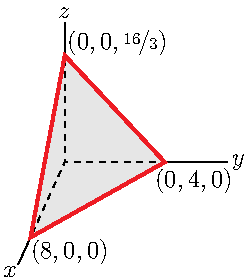
\includegraphics{OE11A_7ai.pdf}
\end{center}
We can use $x$ and $y$ as parameters. As we can rewrite the equation of the
plane as $z = \frac{1}{3}\big(16-2x-4y\big)$, we have
the parametrization
\begin{equation*}
\vr(x,y) = x\,\hi +y\,\hj +\frac{1}{3}\big(16-2x-4y\big)\,\hk
\end{equation*}
In terms of $x$ and $y$, the condition $z= \frac{1}{3}\big(16-2x-4y\big)\ge 0$
is $16-2x-4y\ge 0$ or $x+2y\le 8$. So the domain is
\begin{equation*}
\Set{(x,y)}{x\ge 0,\ y\ge 0,\ x+2y\le 8}
\end{equation*}
Renaming $x$ to $u$ and $y$ to $v$, the parametrization is also
\begin{equation*}
\vr(u,v) = \Big(u\,,\, v\,,\, \frac{1}{3}(16-2u-4v)\Big)\,\hk\qquad
u\ge 0,\ v\ge 0,\ u+2v\le 8
\end{equation*}

(a) (ii) Here is a sketch of the part of the cap in the first octant.
\begin{center}
    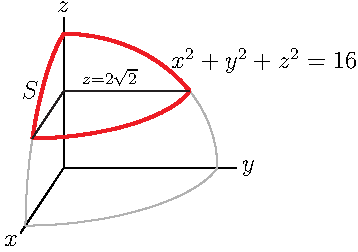
\includegraphics{OE11A_7aii.pdf}
\end{center}
The full sphere can be parametrized (using spherical coordinates with
$\rho=4$) by
\begin{equation*}
\vr(\theta,\varphi) = 4\cos\theta\sin\varphi\,\hi
                     +4\sin\theta\sin\varphi\,\hj
                     +4\cos\varphi\,\hk\qquad
0\le\theta\le 2\pi,\ 0\le\varphi\le \pi
\end{equation*}
In these coordinates, the condition  $4/\sqrt{2} \le z \le 4$ is
\begin{align*}
\frac{4}{\sqrt{2}} \le 4\cos\varphi \le 4
&\iff \frac{1}{\sqrt{2}} \le \cos\varphi \le 1 \\
&\iff 0\le\varphi\le\frac{\pi}{4}
\end{align*}
So our parametrization is
\begin{equation*}
\vr(\theta,\varphi) = 4\cos\theta\sin\varphi\,\hi
                     +4\sin\theta\sin\varphi\,\hj
                     +4\cos\varphi\,\hk\qquad
0\le\theta\le 2\pi,\ 0\le\varphi\le \frac{\pi}{4}
\end{equation*}
Renaming $\theta$ to $u$ and $\varphi$ to $v$, the parametrization is also
\begin{equation*}
\vr(u,v) = \big(4\cos u\sin v\,,\,
                     4\sin u\sin v\,,\,
                     4\cos v\big)\qquad
0\le u\le 2\pi,\ 0\le v\le \frac{\pi}{4}
\end{equation*}

\goodbreak
(a) (iii) Here is a sketch of the hyperboloid.
\begin{center}
    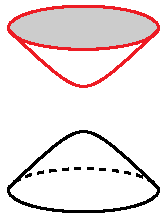
\includegraphics{OE11A_7aiii.pdf}
\end{center}
If we use $x$ and $y$ as parameters, then, since 
$z = \sqrt{1 + x^2 + y^2}$, we have the parametrization 
\begin{equation*}
\vr(x,y) = x\,\hi +y\,\hj +\sqrt{1 + x^2 + y^2}\,\hk
\end{equation*}
In terms of $x$ and $y$, the condition $1\le z\le 10$ is 
\begin{equation*}
1\le \sqrt{1 + x^2 + y^2}\le 10\qquad \text{or}\qquad 0\le x^2+y^2\le 99
\end{equation*}
So the domain is
\begin{equation*}
\Set{(x,y)}{x^2+y^2\le 99}
\end{equation*}
Renaming $x$ to $u$ and $y$ to $v$, the parametrization is also
\begin{equation*}
\vr(u,v) = \big(u\,,\, v\,,\, \sqrt{1 + u^2 + v^2}\big)\qquad
u^2+v^2\le 99
\end{equation*}

Alternatively, if we replace $x$ and $y$ with the polar coordinates
$r$ and $\theta$, we get the parametrization
\begin{equation*}
\vr(r,\theta) = r\cos\theta\,\hi +r\sin\theta\,\hj +\sqrt{1 + r^2}\,\hk
\qquad 0\le\theta\le 2\pi,\ 0\le r\le\sqrt{99}
\end{equation*}
Renaming $r$ to $u$ and $\theta$ to $v$, the parametrization is also
\begin{equation*}
\vr(u,v) = \big(u\cos v\,,\, u\sin v\,,\, \sqrt{1 + u^2}\big)\qquad
0\le v\le 2\pi,\ 0\le u\le\sqrt{99}
\end{equation*}


(b) Let's use the parametrization
\begin{equation*}
\vr(\theta,\varphi) = 4\cos\theta\sin\varphi\,\hi
                     +4\sin\theta\sin\varphi\,\hj
                     +4\cos\varphi\,\hk\qquad
0\le\theta\le 2\pi,\ 0\le\varphi\le \frac{\pi}{4}
\end{equation*}
from part (a) (ii), 
so that
\begin{align*}
\frac{\partial\vr}{\partial\theta}\times\frac{\partial\vr}{\partial\varphi}
&= \det\left[\begin{matrix} \hi & \hj & \hk \\
-4\sin\theta\sin\varphi & 4\cos\theta\sin\varphi & 0 \\
4\cos\theta\cos\varphi & 4\sin\theta\cos\varphi & -4\sin\varphi 
             \end{matrix}\right] \\
&= -16\big(\cos\theta\sin^2\varphi\,,\, \sin\theta\sin^2\varphi\,,\,
                    \sin\varphi\cos\varphi\big)
\end{align*}
and, by (\eref{CLP317}{eq:SUdSparam}) in the CLP-4 text,
\begin{align*}
\dee{S} &= \Big|\frac{\partial\vr}{\partial\theta}\times
            \frac{\partial\vr}{\partial\varphi}\Big|\,\dee{\theta}\dee{\varphi}
= 16\sin\varphi\sqrt{\cos^2\theta\sin^2\varphi
                   + \sin^2\theta\sin^2\varphi
                   +\cos^2\varphi}\,\dee{\theta}\dee{\varphi}  \\
&= 16\sin\varphi\,\dee{\theta}\dee{\varphi}
\end{align*}
So the area is
\begin{align*}
\text{Area}
=\dblInt_S \dee{S}
&=\int_0^{\pi/4}\dee{\varphi}\int_0^{2\pi}\dee{\theta}\ 16\sin\varphi
=32\pi \int_0^{\pi/4}\dee{\varphi}\ \sin\varphi
=32\pi \Big[-\cos\varphi\Big]_0^{\pi/4} \\
&=32\pi\Big[1-\frac{1}{\sqrt{2}}\Big]
\end{align*}
\end{solution}

%%%%%%%%%%%%%%%%%%%%%%%%%%%%%%%
\begin{question}[M317 2017D] %8
Let $S$ be the part of the sphere $x^2+y^2+z^2=2$ where $y\ge 1$, oriented away from the origin.
\begin{enumerate}[(a)]
\item
Compute
\begin{equation*}
\dblInt_S y^3\,\dee{S}
\end{equation*}

\item
Compute
\begin{equation*}
\dblInt_S \big(xy\,\hi + xz\,\hj + zy\,\hk\big)\cdot\hn\,\dee{S}
\end{equation*}
\end{enumerate}
\end{question}

%\begin{hint} 
%\end{hint}

\begin{answer} 
(a) $\frac{\pi}{2}$\qquad
(b) $\frac{\pi}{4}+\frac{2}{3}$
\end{answer}

\begin{solution} 

\emph{Solution 1 --- using tweaked spherical coordinates}.

First we have to parametrize $S$. It is natural
to use spherical coordinates with $\rho=\sqrt{2}$. However if we use
the standard spherical coordinates 
\begin{align*}
x=\sqrt{2}\,\sin\varphi\cos\theta \qquad
y=\sqrt{2}\,\sin\varphi\sin\theta \qquad
z=\sqrt{2}\,\cos\varphi
\end{align*}
the condition $y\ge 1$ becomes $\sin\varphi\sin\theta\ge\frac{1}{\sqrt{2}}$, which is very complicated. So let's back up
and think a bit before we compute. The condition $z\ge 1$, as opposed to 
$y\ge 1$, is easy to implement in spherical coordinates. It is
$\cos\varphi\ge \frac{1}{\sqrt{2}}$ or $0\le\varphi\le\frac{\pi}{4}$.
So let's modify spherical coordinates to make the $y$-axis play the 
role of the $z$-axis, by just exchanging $y$ and $z$ in the parametrization.
\begin{align*}
x=\sqrt{2}\,\sin\varphi\cos\theta \qquad
y=\sqrt{2}\,\cos\varphi\qquad
z=\sqrt{2}\,\sin\varphi\sin\theta
\end{align*}
The condition $y\ge 1$ is then $\sqrt{2}\cos\varphi\ge 1$, which is 
turn is $0\le\varphi\le\frac{\pi}{4}$. Since we have just exchanged 
$y$ and $z$ we could probably just guess $\hn\,\dee{S}$ and $\dee{S}$
from standard spherical coordinates. (See Appendix \eref{CLP317}{ap:spherCoord} in the CLP-4 text and recall that $\rho=\sqrt{2}$.)  But to be on the safe 
side, let's derive them.
We are using the parametrization
\begin{equation*}
\vr(\theta, \varphi) = \sqrt{2}\,\sin\varphi\cos\theta\,\hi
                +\sqrt{2}\,\cos\varphi\,\hj
                +\sqrt{2}\,\sin\varphi\sin\theta\,\hk\qquad
0\le\theta\le 2\pi,\ 0\le \varphi\le \frac{\pi}{4}
\end{equation*}
Since
\begin{align*}
\frac{\partial\vr}{\partial\theta}
&= -\sqrt{2}\,\sin\varphi\sin\theta\,\hi 
           +\sqrt{2}\,\sin\varphi\cos\theta\,\hk \\
\frac{\partial\vr}{\partial\varphi}
&= \sqrt{2}\,\cos\varphi\cos\theta\,\hi - \sqrt{2}\,\sin\varphi\,\hj 
  + \sqrt{2}\,\cos\varphi\sin\theta\,\hk
\end{align*}
so that
\begin{align*}
\frac{\partial\vr}{\partial\theta}\times\frac{\partial\vr}{\partial\varphi}
&= \det\left[\begin{matrix} \hi & \hj & \hk \\[0.05in]
-\sqrt{2}\,\sin\varphi\sin\theta & 0  & 
                 \sqrt{2}\,\sin\varphi\cos\theta \\[0.05in]
\sqrt{2}\,\cos\varphi\cos\theta &- \sqrt{2}\,\sin\varphi & 
                \sqrt{2}\,\cos\varphi\sin\theta
         \end{matrix}\right] \\
&= 2\sin^2\varphi\cos\theta\,\hi +2\sin\varphi\cos\varphi\,\hj 
             + 2\sin^2\varphi\sin\theta\,\hk
\end{align*}
(\eref{CLP317}{eq:SUdSparam}) in the CLP-4 text gives
\begin{alignat*}{3}
\hn\,\dee{S} &= \pm \frac{\partial\vr}{\partial\theta}\times
            \frac{\partial\vr}{\partial\varphi}\,\dee{\theta}\dee{\varphi}
&&= \pm 2\sin\varphi
   \big(\sin\varphi\cos\theta\,,\,\cos\varphi\,,\, \sin\varphi\sin\theta\big)
          \,\dee{\theta}\dee{\varphi} \\
\dee{S} &= \left|\frac{\partial\vr}{\partial\theta}\times
       \frac{\partial\vr}{\partial\varphi}\right|\,\dee{\theta}\dee{\varphi}
&&= 2\sin\varphi \,\dee{\theta}\dee{\varphi}
\end{alignat*}
Choose the plus sign to give the outward pointing normal.

(a)
The specified integral is
\begin{align*}
\dblInt_S y^3\ \dee{S}
&=2\int_0^{\pi/4}\dee{\varphi} \int_0^{2\pi}\dee{\theta}\ 
          \sin\varphi\ \overbrace{\big(\sqrt{2}\,\cos\varphi\big)^3}^{y^3} \\
&=8\sqrt{2}\,\pi \int_0^{\pi/4}\dee{\varphi}\ \sin\varphi\cos^3\varphi \\
&=8\sqrt{2}\,\pi \left[-\frac{\cos^4\varphi}{4}\right]_0^{\pi/4}  \\
&= 2\sqrt{2}\,\pi\left[1-\frac{1}{4}\right]
=\frac{3}{\sqrt{2}}\pi
\end{align*}

(b)
The specified integral is
\begin{align*}
&\dblInt_S \big(xy\,\hi + xz\,\hj + zy\,\hk\big)\cdot\hn\,\dee{S} \\
&\hskip0.25in=
   2\int_0^{\pi/4}\dee{\varphi} \int_0^{2\pi}\dee{\theta}\ \sin\varphi\ 
   \big(2\sin\varphi\cos\varphi\cos\theta\,,\,
      2\sin^2\varphi\sin\theta\cos\theta\,,\,
      2\sin\varphi\cos\varphi\sin\theta\big)\cdot \\&\hskip4.3in
\big(\sin\varphi\cos\theta\,,\,\cos\varphi\,,\, \sin\varphi\sin\theta\big) \\
&\hskip0.25in=
   4\int_0^{\pi/4}\dee{\varphi} \int_0^{2\pi}\dee{\theta}\ 
   \Big\{\sin^3\varphi\cos\varphi\cos^2\theta
        +\sin^3\varphi\cos\varphi\sin\theta\cos\theta
        +\sin^3\varphi\cos\varphi\sin^2\theta
   \Big\} \\
&\hskip0.25in= 4
   \left[\int_0^{\pi/4}\dee{\varphi}\ \sin^3\varphi\cos\varphi\right]
   \left[\int_0^{2\pi}\dee{\theta}\ \big(1+\sin\theta\cos\theta\big)\right] \\
&\hskip0.25in= 4\left[\frac{\sin^4\varphi}{4}\right]_0^{\pi/4}
                 \left[\theta+\frac{\sin^2\theta}{2}\right]_0^{2\pi} \\
&\hskip0.25in= 4\times \frac{1}{16}\times (2\pi)
=\frac{\pi}{2}
\end{align*}

\emph{Solution 2 --- parametrizing by $x$ and $z$}.

We can also parametrize $S$ by using $x$ and $z$ as parameters.
On $S$, 
\begin{itemize}\itemsep1pt \parskip0pt \parsep0pt %\itemindent-15pt
\item[$\circ$]
$y=\sqrt{2-x^2-z^2}$ and
\item[$\circ$]
$y$ runs over the range $1\le y\le\sqrt{2}$. Correspondingly,
$x^2+z^2=2-y^2$ runs over $0\le x^2+z^2\le 1$
\end{itemize}
So we can use the parametrization
\begin{equation*}
\vr(x,z) = x\,\hi +\sqrt{2-x^2-z^2}\,\hj +z\,\hk\qquad
0\le x^2+z^2\le 1
\end{equation*}
Since
\begin{align*}
\frac{\partial\vr}{\partial x}
&= \hi -\frac{x}{\sqrt{2-x^2-z^2}}\,\hj \\
\frac{\partial\vr}{\partial z}
&= -\frac{z}{\sqrt{2-x^2-z^2}}\,\hj  + \hk
\end{align*}
so that
\begin{align*}
\frac{\partial\vr}{\partial x}\times\frac{\partial\vr}{\partial z}
&= \det\left[\begin{matrix} \hi & \hj & \hk \\[0.05in]
1 & -\frac{x}{\sqrt{2-x^2-z^2}}  &  0 \\[0.05in]
0 & -\frac{z}{\sqrt{2-x^2-z^2}} & 1  \end{matrix}\right] \\
&= -\frac{x}{\sqrt{2-x^2-z^2}}\,\hi - \hj 
             -\frac{z}{\sqrt{2-x^2-z^2}}\,\hk
\end{align*}
(\eref{CLP317}{eq:SUdSparam}) in the CLP-4 text gives
\begin{alignat*}{3}
\hn\,\dee{S} &= \pm \frac{\partial\vr}{\partial x}\times
            \frac{\partial\vr}{\partial z}\,\dee{x}\dee{z}
&&= \mp
   \left(\frac{x}{\sqrt{2-x^2-z^2}}\,,1\,,\, \frac{z}{\sqrt{2-x^2-z^2}}\right)
          \,\dee{x}\dee{z} \\
\dee{S} &= \left|\frac{\partial\vr}{\partial x}\times
       \frac{\partial\vr}{\partial z}\right|\,\dee{x}\dee{z}
&&= \sqrt{1+\frac{x^2+z^2}{2-x^2-z^2}}\,\dee{x}\dee{z}
    =\frac{\sqrt{2}}{\sqrt{2-x^2-z^2}}\,\dee{x}\dee{z}
\end{alignat*}
Choose the plus sign to give the outward pointing normal.

(a)
The specified integral is
\begin{align*}
\dblInt_S y^3\ \dee{S}
&=\dblInt_{x^2+z^2\le 1}\dee{x}\dee{z}\ \frac{\sqrt{2}}{\sqrt{2-x^2-z^2}}
          \overbrace{\big(2-x^2-z^2\big)^{3/2}}^{y^3} \\
&=\sqrt{2}\dblInt_{x^2+z^2\le 1}\dee{x}\dee{z}\ \big(2-x^2-z^2\big)
\end{align*}
Switching to polar coordinates with $x=r\cos\theta$ and $z=r\sin\theta$,
\begin{align*}
\dblInt_S y^3\ \dee{S}
&= \sqrt{2}\int_0^{2\pi}\dee{\theta}\int_0^1\dee{r}\ r(2-r^2) \\
&= \sqrt{2}\ (2\pi)\ \left[r^2-\frac{r^4}{4}\right]_0^1
= \sqrt{2}\ (2\pi)\ \left[\frac{3}{4}\right]
=\frac{3}{\sqrt{2}}\pi
\end{align*}

(b)
The specified integral is
\begin{align*}
&\dblInt_S \big(xy\,\hi + xz\,\hj + zy\,\hk\big)\cdot\hn\,\dee{S} \\
&\hskip0.25in=
   \dblInt_{x^2+z^2\le 1}\dee{x}\dee{z}\ 
   \big(x\sqrt{2-x^2-z^2}\,,\,
      xz\,,\,
      z\sqrt{2-x^2-z^2}\big)\cdot \\&\hskip3in
\left(\frac{x}{\sqrt{2-x^2-z^2}}\,,1\,,\, \frac{z}{\sqrt{2-x^2-z^2}}\right) \\
&\hskip0.25in=
   \dblInt_{x^2+z^2\le 1}\dee{x}\dee{z}\ 
   \big\{x^2 +xz +z^2
   \big\} \\
\end{align*}
Switching to polar coordinates with $x=r\cos\theta$ and $z=r\sin\theta$,
\begin{align*}
\dblInt_S \big(xy\,\hi + xz\,\hj + zy\,\hk\big)\cdot\hn\,\dee{S}
&=\int_0^{2\pi}\dee{\theta}\int_0^1\dee{r}\ 
    r(r^2\cos^2\theta +r^2\sin\theta\cos\theta +r^2\sin^2\theta) \\ 
&= 
   \left[\int_0^1\dee{r}\ r^3\right]
   \left[\int_0^{2\pi}\dee{\theta}\ \big(1+\sin\theta\cos\theta\big)\right] \\
&= \left[\frac{r^4}{4}\right]_0^1
                 \left[\theta+\frac{\sin^2\theta}{2}\right]_0^{2\pi} \\
&= \frac{1}{4}\times (2\pi) 
=\frac{\pi}{2}
\end{align*}

\end{solution}

%%%%%%%%%%%%%%%%%%%%%%%%%%%
\begin{question}[M317 1998D] %4
 Let $\cS$ be the part of the surface $(x+y+1)^2+z^2=4$
which lies in the first octant. Find the flux of $\vF$ downwards through
$\cS$ where  
$$
\vF=xy\,\hi+(z-xy)\,\hj
$$
\end{question}

%\begin{hint} 
%\end{hint}

\begin{answer} 
$-\frac{5}{6}$
\end{answer}

\begin{solution} 
First observe that, 
\begin{itemize}\itemsep1pt \parskip0pt \parsep0pt %\itemindent-15pt
\item[$\circ$]
because $(x+y+1)^2\ge 0$,
 all points on $(x+y+1)^2+z^2=4$ have $|z|\le 2$ 
and that, 
\item[$\circ$]
for $|z_0|\le 2$, the surface $(x+y+1)^2+z^2=4$
intersects the horizontal plane $z=z_0$ on $(x+y+1)^2 = 4-z_0^2$,
i.e. on the two lines $x+y=\pm\sqrt{4-z_0^2}-1$, $z=z_0$.
\item[$\circ$]
The line $x+y=\pm\sqrt{4-z_0^2}-1$, $z=z_0$
intersects the first octant if and only if $z_0\ge0$ and
$\pm\sqrt{4-z_0^2}-1\ge 0$. 
\item[$\circ$]
Thus $x+y=-\sqrt{4-z_0^2}-1$, $z=z_0$ never intersects the first octant and
\item[$\circ$]
 $x+y=\sqrt{4-z_0^2}-1$, $z=z_0$
intersects the first octant if and only if $0\le z_0\le \sqrt{3}$.
\item[$\circ$] When $z_0=0$, the line $x+y=\sqrt{4-z_0^2}-1$, $z=z_0$
is $x+y=1$, $z=0$.
\item[$\circ$] When $z_0=\sqrt{3}$, the line $x+y=\sqrt{4-z_0^2}-1$, $z=z_0$
is $x+y=0$, $z=2$.
\item[$\circ$] So as $(x,y,z)$ runs over $\cS$, $(x,y)$ runs over the
triangle $x\ge0$, $y\ge 0$, $x+y\le 1$.
\end{itemize}
Let $G(x,y,z)=(x+y+1)^2+z^2$. Then
$$
\hn\,\dee{S}=\pm\frac{\vnabla G}{\vnabla G\cdot\hk}\ \dee{x}\dee{y}
=\pm\frac{2(x+y+1)\hi+2(x+y+1)\hj+2z\hk}{2z}\,\dee{x}\dee{y}
$$
For the downward normal, we need the minus sign, so
\begin{align*}
\vF\cdot\hn\,\dee{S}
&=-\big[xy\,\hi+(z-xy)\,\hj\big]\cdot
  \Big[\frac{(x+y+1)\hi+(x+y+1)\hj+z\hk}{z}\Big]\,\dee{x}\dee{y}\\
&=-\frac{1}{z}\big[xy(x+y+1)+(z-xy)(x+y+1)\big]\,\dee{x}\dee{y}\\
&=-\frac{1}{z}\big[z(x+y+1)\big]\,\dee{x}\dee{y}\\
&=-(x+y+1)\,\dee{x}\dee{y}
\end{align*}
The domain of integration is $x\ge 0,\ y\ge 0,\ x+y\le 1$, so
\begin{align*}
\dblInt_\cS\vF\cdot\hn\,\dee{S}
&=-\int_0^1 \dee{x}\int_0^{1-x} \dee{y} \ (x+y+1)
=-\int_0^1 \dee{x}\ \Big[(1+x)(1-x)+\frac{1}{2}(1-x)^2\Big]\\
&=-\int_0^1 \dee{x}\ \Big[\frac{3}{2}-x-\frac{1}{2} x^2\Big]
=-\Big[\frac{3}{2}-\frac{1}{2}-\frac{1}{6}\Big]
=-\frac{5}{6}
\end{align*}
\end{solution}
